\section{Definition and general properties of the fundamental
  group}\label{sec1} % sec 1.  

We\pageoriginale call a continuous map simply a map. We denote the
real line by $\mathbb{R}$ and the unit interval by $I$:  
$$
I= \{t|t \in \mathbb{R}, 0 \leq t \leq 1\}.
$$
We consider maps of $I$ into a topological space $X$ and say that a
map $f_1$ is equivalent to a map $f_2$ if there exists an automorphism
$\varphi$ of $I$ fixing end points such that $f_1=f_2 \circ  \phi$. This is an
equivalence relation in the set of all maps of $I$ into $X$. An
equivalence class under this relation is called a \textit{path} in
$X$. We say that a map $f$ \textit{defines a path} $W$ if $f$ belongs
to the equivalence class $W$. Clearly any two maps defining the same
path map 0 onto the same point and also 1. The images of 0 and 1
are called the \textit{initial} and the terminal point of the path. We
say that a path connects a point $x$ to a point $y$ if $x$ and $y$
are the initial and terminal points of the path. 

Suppose that a map $f$ defines a path $W$ connecting  $x_0$ to
$x_1$. Then the map 
$$
f^{-1}(t) = f(1-t),  \quad 0 \leq t \leq 1  
$$
defines a path $W^{-1}$ which can be seen to be dependent only on
$W$. This path connecting $x_1$ to $x_0$ is called the path $W$
described in the opposite sense or the reversed path of $W$. 

If $C$ is a Jordan arc, i.e. a set homeomorphic to $I$, there are two
paths defines by homeomorphism of $I$ onto $C$, each reversed to the
other, and corresponding to the two orientations of $C$.  

\medskip
\noindent
\textbf{The\pageoriginale product of paths.}

Let $f_1$ and $f_2$ be two maps of $I$ into $X$ such that
$f_1(1) = f_2(0)$. Then we can define a new map $f_1f_2$ by setting  
$$
f_1 f_2 (t)=
\begin{cases}
f_1 (2t) & \text { if } 0 \leq t \leq \frac{1}{2},\\
f_2 (2t-1) & \text { if }\frac{1}{2} \leq t \leq 1.
\end{cases}
$$

If $g_1$ and $g_2$ are equivalent to $f_1$ and $f_2$ respectively and
the equivalences are give by the automorphisms $\varphi_1$ and
$\varphi_2$ of $I$;  
$$
f_1=g_1 \circ \varphi_1, f_2=g_2 \circ \varphi_2 
$$
then the automorphism
$$ 
\varphi (t)=
\begin{cases}
\frac{1}{2} \varphi_1(2t) & \text{ if } 0 \leq t \leq \frac{1}{2},\\ 
\frac{1}{2} +\frac{1}{2} \varphi_2(2t-1) & \text{ if } \frac{1}{2}
\leq t \leq 1 
\end{cases}
$$
defines an equivalence between $f_1 f_2$ and $g_1 g_2$:
$$
f_1 f_2 =(g_1 \circ  \varphi_1) (g_2 \circ  \varphi_2) = g_1 g_2 \circ
\varphi.  
$$
Hence the path defined by $f_1 f_2$ depends only on the paths $W_1$ and
$W_2$ defined by $f_1$ and $f_2$. This path is called the product of
the paths $W_1$ and $W_2$ and is denoted by $W_1 W_2$. 
This product is associative. For suppose that
$W_1, W_2$ and $W_3$ are paths defined by the maps $f_1$, $f_2$ and
$f_3$ such that 
$$
f_1 (1)=f_2(0) \text{~ and~ } f_2 (1)=f_3(0). 
$$
Then, if $\varphi$ is the automorphism of $I$ taking the points 0,
$\dfrac{1}{4}$, $\dfrac{1}{2}$ and 1 onto the points $0$,
$\dfrac{1}{2}$, $\dfrac{3}{4}$ and 1 respectively and which is
linear on\pageoriginale the intervals $[0,\dfrac{1}{4}]$, $
[\dfrac{1}{4},\dfrac{1}{2}]$ and $[\dfrac{1}{2}, 1]$, we have  
$$
f_1(f_2 f_3) \circ  \varphi= (f_1 f_2)f_3 
$$
and hence $W_1(W_2 W_3)= (W_1 W_2)W_3$. 

It is clear that each subdivision of the unit interval gives rise to a
representation of a given  path as a product of paths and by passing
to a sufficiently fine subdivision of $I$ we can represent that given
path as the product of paths which are as small as we wish. 

\medskip
\noindent
\textbf{Homotopy of paths.}
 Two maps $f$ and $g$ of $I$ into $X$ are
\textit{homotopic with fixed end points} if there exists a continuous
family of maps $f_t:I \to X (0 \leq t \leq 1)$ such that $f_0=f$,
$f_1=g$ and $f_t(a)=f(0)$, $f_t(1)=f(1)$. The family $f_t$ is said to
be continuous if the map $F:I \times I \to X$, defined by $F
(s,t)=f_t(s)$, is continuous. We then say that $f_t$, or $F$, is a
\textit{homotopy form} $f$ \textit{to} $g$. This is an equivalence
relation, for it is 
\begin{enumerate}[(i)]
\item reflexive : the family $f_t=f$ defines a homotopy from $f$ to
  $f$.

\item symmetric : if $f_t$ defines homotopy from $f$ to $g$ then
  $f_{1-t}$ defines homotopy from $g$ to $f$. 

\item transitive : if $f_t$ and $g_t$ define homotopies from $f$ to
  $g$, and $g$ to $h$ respectively then the family 
$$
h_t= 
\begin{cases}
f_{2t} & 0 \leq t \leq \frac{1}{2},\\
g_{2t-1} & \frac{1}{2} \leq t \leq 1
\end{cases}
$$
defines a homotopy from $f$ to $h$. This relation is denoted by $\approx$.
\end{enumerate}

Every\pageoriginale map $\varphi:I \to I$ fixing end points is
homotopic to the 
identity, for $\varphi_t(s)=ts+(1-t)\varphi (s)$ is such a
homotopy. If $f=g\circ\varphi$, then $f_t=g\circ\varphi_t$ is a homotopy
from g to $f$. Hence, if two maps define the same path, they are
homotopic (with fixed end pints). Hence, all maps defining the same
path $w$ belong to the same class, which will be denoted by $[w]$,
and we get an equivalence relation in the set of paths in $X$, which
we still call homotopy and denote by $\approx$. 

It is clear that if two paths are homotopic, then they have the same
initial point and the same terminal point. If the product $w_1 w_2$ is
defined, i.e. if the terminal point of $w_1$ is the initial point of
$w_2$, one sees that $[w_1 w_2]$ depends only on $[w_1]$ and
$[w_2]$. We then call $[w_1 w_2]$ \textit{the product of} $[w_1]$ and
$[w_2]$ and we write $[w_1][w_2]=[w_1w_2]$. 

We denote the set of homotopy classes of paths in $X$ having the same
point $x_0$ as initial and terminal point by $\pi (X,x_0)$. In this
set the operation of forming products is defined for every pair of
elements. Now we prove that this set form a group with respect to this
operation. We have already proved that the operation is associative
and if remains to prove the existence of a unit element and inverse. 

Let $e$ be the path reduced to $x_0$, defined by the constant map
$e(s)=x_0$, and let $w$ be any path closed at $x_0$, defined by the
map $f$. Then 
$$
f_t(s)=
\begin{cases}
f (\frac{2s}{1+t}) & \text{ for } 0 \leq s \leq \frac{1+t}{2}\\
e(s)=x_0 &\text{ for} \frac{1+t}{2} \leq s \leq t
\end{cases}
$$\pageoriginale
is a homotopy from $fe$ to $f$. There is a similar homotopy from $ef$ to
$f$. Hence $[w][e]=[e][w]=[w]$ and $[e]$ is a unit element. 

Now, for any path $w$ with initial points $x_0$, we have
$[ww^{-1}]=[e]$. For, if $w$ is defined by $f$, 
$$
g_t(s)=
\begin{cases}
f(2st) & \text{ for } 0 \leq s \leq \frac{1}{2},\\
f((2-2s)t) & \text{ for } \frac{1}{2} \leq s \leq 1
\end{cases}
$$
is a homotopy from $e$ to $ff^{-1}$, hence $[ww^{-1}]=[e]$. If $w$ is
closed at $x_0$, we have also $[w^{-1}w]=[e]$, so that
$[w^{-1}][w]=[w][w^{-1}]=[e]$ and $[w^{-1}]$ is an inverse $[w]^{-1}$
to $[w]$.  

The group $\pi(X,x_0)$ is called the \textit{fundamental group of
  $X$ based at $x_0$}. 


Suppose that $x_0$ and $x_1$ are points of $X$ connected by the path,
$L$, and consider the map $J_L: \pi (X,x_0) \to \pi (X, x_1)$ defined by
$J_L[w]=[L^{-1}wL]$. It is an homomorphism, for
\begin{align*}
J_L[w_1]J_L[w_2] &= [L^{-1}w_1 LL^{-1} w_2 L]=[L^{-1}w_1][LL^{-1}][w_2
  L]\\
&=[L^{-1}w_1 w_2L]=J_L [w_1][w_2].
\end{align*}
Further, $J_{L^{-1}} : \pi
(X,x_1) \to \pi (X,x_0)$ is an inverse to $J_L$, so that $J_L$
\textit{is an isomorphism}. It is clear that it depends only on $L$. 

If $L'$ is another path connecting $x_0$ to $x_1$, we have
$[L']=[L'L^{-1}L]=[CL]$ with $C=L'L^{-1}$ closed at $J_{L'}$
$[w]=[L^{-1}C^{-1}wCL]=J_L\circ J_C [w]$\pageoriginale where $J_C$ is an inner
automorphism of $\pi (X,x)$. Hence $J_{L'}$ and $J_L$ differ only by
an inner automorphism. 

Now suppose that the space $X$ is arcwise connected. Then it follows
that $\pi (X,x)$ for various $x$ in $X$ are isomorphic to each other
and hence determine a group $\pi (X)$, called \textit{the
  fundamental group of} $X$. But there are in general no canonical
isomorphisms between the various $\pi (X,x)$, these isomorphisms
being determined up to an inner automorphism. In case $\pi (X)$ us
abelian, they are consequently determined in a canonical manner. 

A space is called simply connected if it is connected and its
fundamental group is trivial. 

A convex set in the euclidean space is simply connected: A subset $E$
of $\mathbb{R}^n$ is convex if the line segment connecting any two of
its points is in $E$: 
$$
x \in E, y \in E \text{ implies } (1-t)x+ty \in E; 0 \leq t \leq 1.
$$

Thereby it follows that any two paths connecting the same points are
homotopic, and the set is simply connected. 

The simplest example of a space which is not simply connected is the
circle. We shall prove this fact later. 


Now, suppose $X$ and $Y$ are two spaces and $\mu :X \to Y$ is a
map. If $w$ is a path in $X$ defined by $f$, the $\mu\circ f$ defines a
path in $Y$, which is called \textit{the image of $w$ by $\mu$}, and
denoted by\pageoriginale $\mu(w)$ or $\mu w$. It is clear that $\mu
(w_1 w_2)=\mu 
(w_1)\mu(w_2)$ and if $w \approx w^1$, $\mu(w) \approx \mu
(w')$. There follows that, if $y_0= \mu (x_0)$, we have a homomorphism 
$$
\mu_\ast: \pi (X,x_0) \to \pi (Y,y_0)
$$ 
defined by $\mu_\ast [w]= [\mu w]$. We call $\mu_\ast$ the homomorphism
induced by $\mu$. 

If $\mu_0$ and $\mu_1$ are maps of $X$ into $Y$, a homotopy from
$\mu_0$ to $\mu_1$ is a continuous family of maps $\mu_t:X \to Y(0
\leq t \leq 1)$. That means that $M(x,t)=\mu_t (x)$ is a continuous
map of $X \times I$ into $Y$.  

\begin{theorem}\label{thm1.1}% Thm 1.1
If $\mu_t: X \to Y$ is a homotopy from $\mu_0$ to $\mu_1$, and if
  $L$ is the path connecting $y_0=\mu_0 (x_0)$ to $y_1=\mu_1(x_0)$ in
  $Y$, defined by $\mu_t (x_0)$, then $\mu_{1\ast}=J_L\circ \mu_{0\ast}$. 
\end{theorem}

\begin{proof}
Suppose $w$ is a path closed at $x_0$, define by the map $f: I \to
X$. Then $\mu_0 w$ is the image of $I \times 0=(0 \leq s \leq 1,t=0)$
by the map $M: I \times I \to Y$, where $M(s,t)=\mu_t\circ f(s)$. The
image of the other sides of the square $I \times I=(0 \leq s,t \leq
1)$ are $L$, $\mu_1 w$ and $L^{-1}$. As the square is simply connected
(as a convex set), $I \times 1$ is homotopic to the path with same end
points made of the three other sides, their images are also homotopic,
i.e. 
$$
\mu_1 w \approx L^{-1} (\mu_0 w) L \quad \text{and} \quad  \mu_{1\ast}
   [w] = J_L \mu_{o\ast} [w]  
$$
\begin{figure}[H]
\centering
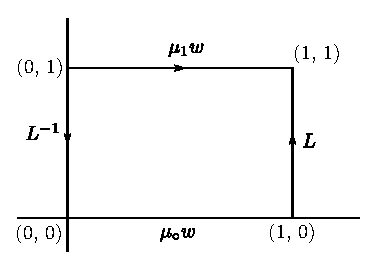
\includegraphics{vol44-fig/fig44-1.eps}
\end{figure}
\end{proof}

\begin{corollary}\label{cor1}% 1
If\pageoriginale a map $\mu :X \to X$ is homotopic to the identity map
of $X$ onto 
itself then $\mu_*$ is an isomorphism. Further if the homotopic leaves
the base point $x_0$ fixed then the isomorphism coincides with the
identity isomorphism since in this case $L$ reduces to $x_0$. 
\end{corollary}

A map $\mu:X \to Y$ is called a \textit{homotopy equivalence} if there
exists a map $\lambda :Y \to X$ such that 
$$
\mu\circ\lambda \approx \id_Y \text{ and } \lambda\circ\mu \approx \id_X.  
$$

A subspace $Y$ of $X$ is called a deformation retract of $X$ if the
inclusion map of $Y$ into $X$ is a homotopy equivalence. 

With these definitions we have the following:

\begin{corollary}\label{cor2}%2
If $\mu:X \to Y$ is a homotopy equivalence and $X$ is arcwise
connected then 
$$
\pi (X) \simeq \pi (Y). 
$$
\end{corollary}

\begin{corollary}\label{cor3} %3
If $Y \subset X $ is a deformation retract of $X$ then 
$$
\pi (X) \simeq \pi (Y).
$$
\end{corollary}

\begin{theorem}\label{thm1.2} %(1.2)
Suppose that $X$ and $Y$ are arcwise connected spaces and $x_0$ is in
$X$ and $y_0$ is in $Y$. Then 
$$
\pi (X \times Y, (x_0,y_0)) \simeq \pi(X,x_0) \times \pi
(Y,y_0). 
$$
in a canonical manner.
\end{theorem}

\begin{proof}
We denote the projection of $X \times Y$ onto $X$ by $p_1$ and the
other projection by $p_2$: 
$$
p_1 (x,y) = X, \quad p_2(x,y)= y 
$$
and\pageoriginale thus have homomorphisms $P_{1\ast}$ and
$P_{2\ast}$. Hence we have a homomorphism 
$$
\pi (X \times Y, (x_0,y_0)) \xrightarrow{(P_{1 \ast},P_{2 \ast})} \pi 
(X,x_0) \times \pi (Y,y_0). 
$$

Suppose that $w_1$ and $w_2$ are closed paths in $X$ and $Y$ around
$x_0$ and $y_0$ respectively defined by $f$ and $g$. Then denoting the
path defined by the map 
$$
t \longmapsto (f(t),g(t)) 
$$
by $w$ we have
$$
(P_{1\ast}, P_{2\ast}) (W)=(W_1,W_2)
$$
and hence $(P_{1 \ast}, P_{2\ast})$ is surjective.

Suppose that $W \in \pi (X \times Y, (x_0,y_0))$ is such that
$P_{1\ast}W$ and $P_{2\ast}W$ are unit elements and the homotopies are given
by maps $F_1$ and $F_2$ respectively. Then the map 
$$
(s,t)\longmapsto (F_1 (s,t),F_2 (s,t)) 
$$
gives a homotopy between $W$ and the constant path at $(x_0,y_0)$ of
$X \times Y$. Hence $(P_{1\ast}, P_{2 \ast})$ is injective. 
\end{proof}

\section{Free products of groups and their quotients}\label{sec2} %2

Suppose\pageoriginale that $\{ G_i \}_{i \in I}$ is a family of groups
and that the elements of $G_i$ for different $i$ are distinct. We
denote the union of the $G_i$ by $E$ and associated $W(E)$ to it. The
elements of $W(E)$, called \textit{words}, are finite sequences $W$
of elements from $E$:  
$$
W=a_1 a_2 \cdots a_n ; \;\; a_i \in E 
$$
The integer $n$ is called the \textit{length} of the word $W$ and is
denoted by $lg(W)$. The unique word whose length is zero is called the
empty word and is denoted by $W_0$. Each element of $E$ gives rise to
a unique word of length one and conversely. Therefore we identify $E$
with the subset of $W(E)$ consisting of words of length one. Now if 
$$
W=a_1 a_2 \cdots a_m \text{ and } W'=a'_1a'_2 \cdots a'_n
$$
are two words then we define the product of $W$ and $W'$, denoted by
$WW'$, by the equation $WW'=a_1 a_2 \cdots a_m a'_1a'_1 \cdots
a'_n$. This product is associative and it is clear that the empty
word is the unit element with respect to this operation. Hence the set
$W(E)$ is a semigroup. Since $lg WW'=lg W+ lgW'$ no word expect $W_0$
has an inverse. 

Now we introduce a relation in $W(E)$. We say that \textit{two words
  are equivalent} if one can be changed into the other by means of a
finite number of operations of the following kind: 
\begin{enumerate}[(a)]
\item Deletion\pageoriginale from the word of an element $e$ which is
  the unit element of some $G_i$, or introduction of such a unit
  element:  
$$ 
A eB \rightleftarrows AB.
$$

\item Replacement of two consecutive elements $x$, $y$ belonging to
  the same group $G_i$ by the element $z$ equal to their product in
  $G_i$ or replacement of $z$ by $xy$: 
$$
A xyB \rightleftarrows AzB. 
$$
\end{enumerate}

\noindent
If the word $W$ and $W'$ are equivalent we write $W \sim W'$. This is
an equivalence relation. We denote the equivalence class containing
the empty words $W_0$ by $W_0$ itself. Then it directly follows that
the operation of forming products passes down to the quotient set
$W(E)/W_0$ of equivalence classes, i.e. if $W_1 \sim W'_1$ and $W_2
\sim W'_2$, then $W_1 W_2 \sim W'_1 W'_2$. Hence $W(E)/W_0$ is a
semigroup. We assert that it is a group. For this we define the
\textit{reverse} of a word. If $W=a_1 a_2 \cdots a_n$, the reverse of
$W$, denoted by $W^{-1}$ is $a^{-1}_n a^{-1}_{n-1} \cdots a^{-1}_2
a^{-1}_1$. For any words $W$ and $W'$ we have $(WW')^{-1}=W'^{-1}
W^{-1}$, $(W^{-1})^{-1}=W$ and $W^{-1}_0 =W_0$. 

Now suppose that $W$ is a words of length $n$. If we apply (b) and (a)
successively $n$-times to $WW^{-1}$, we see that $WW^{-1}$ is equivalent
to the unit element $W_0$, and also that so is $W^{-1}W$. Hence
$W(E)/W_0$ is a group. 

The above group is called the \textit{free product} of the family of
groups $G_i$. It is denoted by $\underset{i}{\ast}G_i$ and if $I$ is a
finite set of $n$ elements then it is also denoted by  
$$
G_{i_1} \ast G_{i_2} \ast  \ldots  \ast G_{i_n}.
$$\pageoriginale
The $G_i$ are called the factor of $\underset{i}{\ast} G_i$.

\begin{defi*}
A word $W=a_1 a_2 \cdots a_n$ is called {\em reduced} if  
\begin{enumerate}[(i)]
\item No $a_i$ is the unit element of some $G_{i(W)}$. 

\item No two consecutive elements $a_i$, $a_{i+1}$ belongs to the same
  group $G_i$.
\end{enumerate}

The simplest example of a reduced word is an element
 $x$ of $E$ different from the units of $G_i$. 
\end{defi*}

\begin{theorem}\label{thm2.1}%% 2.1
Each equivalence class of $W(E)$ contains one and only one reduce word.
\end{theorem}

\begin{proof}
For every reduced word $w=a_1 a_2 \cdots a_r$ and every $a \in E$, we
get a reduced word $|aw|$ equivalent to $a w$ by setting  
$$
|aw|=
\begin{cases}
a_1 a_2 \cdots a_r & \text{ if a is a unit element}\\
aa_1a_2 \cdots a_r & \text{ if a is not a unit element}\\
& \text{ and does not belong to the same }\\
& \text{ $G_i$ as $a_i$}\\ 
ba_2 \cdots a_r & \text{ if a belongs to the same $G_i$ }\\
& \text{ as $a_1$ and $aa_1=b$ is not}\\
& \text{ a unit element}\\ 
a_2 \cdots a_r  & \text{ if } a=a^{-1}_1.
\end{cases}
$$
By induction on the length, one proves that every word is equivalent 
to at least one reduced word. 

To prove the unicity, following an idea of Van der Waerden, let us
denote by $T(a)$,  for every $a \in E$, the map of the set of all
reduced words into itself which changes $w$ into $|aw|$, and for any
word $W_1=b_1 b_2 \cdots b_s$, reduced or not, let us set
$T(w_1)=T(b_1)T(b_2) \cdots T(b_r)$.\pageoriginale It can be easily
verified that, 
if $a$ and $b$ belong to the same $G_i$ and $ab=c$, then
$T(c)=T(a)T(b)$, while $T(e)=$identity if $e$ is a unit
element. There follows that if the words $w_1$ and $w_2$ are
equivalent, $T(w_1)=T(w_2)$. Now, a reduced word $w$ is the image of
the empty word $W_0$ by $T(w)$. Hence, if $w_1$ and $w_2$ are
equivalent reduced words, they are the images of $W_0$ by the same
map, $w_1=w_2$, which proves the unicity. 

If $x \in G_i$ is not the unit element of $G_i$, then it is a reduced 
word. If we map the unit element of each $G_i$ onto the empty word of
$W(E)$ and the other by inclusion into  $W(E)$ we obtain an
isomorphism of $G_i$ onto a subgroup of $\underset{i}{\ast} G_i$; let us
identify $G_i$ with the corresponding subgroup. With this
identification it is clear that 
$$
G_i \cup G_j =W_0 \text{ for } i \neq j.
$$
\end{proof}

\begin{theorem}\label{thm2.2}%%% 2.2
Given a group $G$, a family $G_i$ of groups and a family of
  homomorphisms 
$$
h_i:G_i \to G
$$
then there exists one and one homomorphism $h$ of $\underset{i}* G_i$
onto $G$ such that 
$$
h|G_i =h_i.
$$
\end{theorem}

\begin{proof}
For the proof it is better to consider the semigroup $W(E)$. Given any
map $g$ of $E$ into a semigroup $G$ then we can extend it into a
homomorphism $g^\ast$ of $W(E)$ into $G$ by setting  
$$
g^\ast (a_1 a_2 \cdots a_n)=g(a_1)g(a_2)\cdots g(a_n).
$$
for\pageoriginale every word $a_1a_2 \cdots a_n$. Further if $g$ is
given by a 
family $h_i$ of homomorphisms of $G_i$ into $G$ then equivalent
elements of $W(E)$ go into the same element of $G$ under the map $g^\ast$
(This fact can be proved by induction on the number of operations (a)
and (b) performed to change a word into its equivalent). Hence $g^\ast$
gives a homomorphism of $\underset{i}{\ast} G_i$ onto $G$. The uniqueness
part is clear because any homomorphism $g^\ast_1$ of $\underset{i}{\ast} G_i$
which equal $g_i$ on $G_i$ has to satisfy the defining equation of
$g^\ast$. Hence the result. 
\end{proof}

\medskip
\noindent
\textbf{The quotient of a free product by a set of relations.}

Suppose we are given a family $(S_j,T_j)_{j \in J}$ of pairs of words
of $W(E)$, and consider the set of relations $R=\{ S_j=T_j \}_{j \in
  J}$. We say that two words are $R$-equivalent if one can be changed
into the other by a finite number of operations (a), (b) and 

(c) ~ Replacement of $S_j$ by $T_j$ or $T_j$ by $S_j$ at will. If two
words $W$, $W'$ are $R$-equivalent we write 
$$ 
W_{\underset{R}{\sim}} W'
$$
It is a matter of direct verification that $R$-equivalence is an
equivalence relation. We denote the equivalence class determined by
the empty word $W_0$ by $W_R$ and it follows directly that the product
operation in $W(E)$ passes down to the quotient set $W(E)/ W_R$ of the
equivalence classes. (This fact can be proved by\pageoriginale
induction on the 
number of operation (a), (b), (c) used to changed a word into its
equivalent). Since the operations (a) and (b) are subsumed under
$R$-equivalence it follows that $R$-equivalence can be considered as an
equivalence ration in $\underset{i}{\ast} G_i$ and that $W(E)/W_R$ can be
considered as the set of equivalence classes of $\underset{i}{\ast} G_i$
under $R$. It follows that $W(E)/W_R$ is a group. This group is called
\textit{the quotient group of the free product $\underset{i}{\ast} G_i$ by
  the set of relations $R$}. 

We say that two sets $R$ and $R'$ of relations in $W(E)$ are
equivalent if $R$-equivalence implies and is implied by $R'$-equivalence,
i.e. for any two words $W$ and $W'$ we have $W_{\underset R {\sim}
}W'$ if and only if $W_{\underset R  \sim }W'$. In this case we write
$R \sim R'$. 

\begin{example*}
Consider $R=\{ S_j=T_j \}$ and $R'= \{ S_j T^{-1}_j=W_0 \}$ then we
have $R \sim R'$. 

A set of relations $S_j=W_0$ is also written $S_j=1$ and the $S_j$ are
sometimes called relaters. 
\end{example*}

\begin{defi*}
A {\em free group} is the free product of a family of groups each of
which is infinite cyclic. 
\end{defi*}

Suppose that we are given a group $G$ and a system $\{ a_i \}_{i \in
  I}$ of generations of $G$. Suppose that $Z$ denotes the infinite
cyclic group and $e$ a generator of $Z$ and that we denote the
homomorphism of $Z$ into $G$ taking $e$ onto $a_i$ by $h_i$. Now if we
take copies $Z_i$ of $Z$ one for each $i$ in $I$ and form the free
product, by theorem \ref{thm2.2}. there exists a homomorphism $h$
of\pageoriginale 
$\underset{i}{\ast} Z_i$ into $G$ such that $h|G_i=h_i$. This homomorphism
is not since a system $\{ a_i \}_{i \in I}$ of generators of $G$ is in
the image. Hence $G$ is isomorphic to the quotient of $\underset{i}{\ast}
Z_i$ by the kernel of $h$. Hence each group can be represented as a
quotient of a free group. The word in the kernel give a set of
relators for $G$. 

\begin{theorem}\label{thm2.3} % them 2.3
Suppose that $W \neq W_0$ is an element of finite order in
  $\underset{i}* G_i$. Then there is one and only one $i$ in $I$ such
  that $W$ is conjugate to an element of $G_i$. 
\end{theorem}

\begin{proof}
Among the reduced words corresponding to the conjugates $W_1\break WW^{-1}_1$
suppose that $W'=W_1 W W^{-1}_1$ is one length and that 
$$
W'=a_1a_2 \cdots a_r.
$$
\end{proof}

To prove the result we first show that $r=1$. Suppose that $r
>1$. Then $a_1$ and $a_r$ do not belongs to the same group for if they
belong to the same group then the conjugate 
$$
a^{-1}_ra_1a_2 \cdots a_{r-1}=a'_1a_2 \cdots a_{r-1} 
$$
of $W$ would have length $r-1$ contradicting the minimality of
$r$. But if $a_1$ and $a_r$ are not in the same group, then $(W')^n$
is reduced for every $n$, therefore $W^n$ is never the unit element
$W_0$. Hence $r=1$ and there is an $i$ such that $G_i$ contains a
conjugate of $W$. The unicity follows from the fact that every
conjugate of $a_1$ is represented by a reduced word of the form $Aa'
A^{-1}$ with $a' \in G_i$. 

\begin{theorem}\label{thm2.4} %2.4
The\pageoriginale center of a free group $G=\underset{i}{\ast} G_i$
 with at least two factors is trivial i.e. consists of $W_0$ alone. 
\end{theorem}

\begin{proof}
Suppose that $a_1a_2 \cdots a_r$ is a reduced word in the center of
the group. Suppose that $a_1$ is in $G_i$. Then since $G$ contains at
least two factors there is a group $G_j$ different from $G_i$, let $a$
be an element of $G_j$ different from the unit. Then the word $aa_1
\cdots a_r$ is a reduced word; further the word $a_1 a_2 \ldots a_r a$
is reduced if $a_r$ and $a$ do not belong to the same
group $G_j$, otherwise $a_1a_2 \cdots a_r a$ has length $r$, hence
$a_1a_2 \cdots a_r a \neq a_1a_2 \cdots a_r$; in each case $a_1a_2
\cdots a_r a$ then $a_1a_2 \cdots a_r a$ represent distinct equivalent
classes, a contradiction. 
\end{proof}

\begin{theorem}\label{thm2.5}%2.5
The quotient of a free product $G=\underset{i}* G_i$ of abelian
  group by the commutator subgroup $G'$ is isomorphic to the direct
  sum $\underset{i}\times  G_i$. 
\end{theorem}

\begin{proof}
The direct sum $\underset{i}\times G_i$ is the subgroup of the direct
product of the $G_i$ consisting of the families $(a_i)_{i\in I}$ where
all $a_i$ but for a finite number are unit elements. By theorem \ref{thm2.2},
there is a homomorphism  
$$
h:\underset{i}\ast G_i \to \underset{i}\times G_i
$$
such that $h|G_i$ is the canonical injection of $G_i$ into
$\underset{i}\times G_i$. Since $\underset{i}\times G_i$ is abelian ($G$ is
assumed abelian), $G'$ is in the kernel of $h$. Hence we have the
natural maps 
$$
G \xrightarrow{p} G/G' \xrightarrow{\bar{h}} \underset{i}\times G_i 
$$
with $h=\bar{h} op$.
\end{proof}

Now,\pageoriginale suppose that $a=a_1a_2 \cdots a_m$ is in the kernel
of $h$, where 
$a_1, a_2, \cdots, a_m $ are elements of $\bigcup\limits_{i=1}^n
G_i$. Let $A_k$ be the product of the $a_i$ which belongs to $G_k$,
and $A=A_1A_2 \cdots A_n$. Then $p(A)= p(a)$ and $h(A) = h(a) =
1$. Because $h(A) = (A_i)_{i \in I}$, where $A_i$ is 
for $i> n$ the unit element of $G_i$, this implies that $A=1$,
$p(a)= 1$ and $a \in G'$. Hence $G'$ is the kernel of $h$. 

\begin{theorem}\label{thm2.6} %2.6
If two free products of cyclic groups are isomorphic, then their
factors are the same. 
\end{theorem}

\begin{proof}
Let $G = \underset{i}\ast G_i$ and $G'=\underset{j}\ast G'_j$. be two free
products of cyclic groups, which are isomorphic. For $1 < k \leq
\infty$, let $N_k (\resp N'_k$) be the number of the $G_i(\resp G'_j)$
which are of order $k$. We prove that $N_k=N'_k$. For $k= \infty$,
$N_\infty$ is the rank of $\underset{i}\times G_i$ and $N'_\infty$ of 
rank of $\underset{j}\times G'_j$. According to theorem \ref{thm2.5},
$\underset{i}\times G_i$ and $\underset{j}\times G'_j$ are
isomorphic, hence $N_\infty = N'_\infty$. For $k$ finite $>1$, let us
consider the cyclic subgroup of $G$ of order $k$ which are maximal,
i.e. not contained in a larger cyclic subgroup. From theorem \ref{thm2.3}, it
follows that such maximal subgroup is conjugate to one and only one
$G_i$. Hence $N_k$ is the number of conjugacy classes of maximal
cyclic subgroups of $G$ of order $k$. Therefore, the isomorphism of
$G$ and $G$, implies $N_k= N'_k$. 

If $G$ is the quotient of a free group generated by $a_1, a_2,
\ldots$ by the set of relations $S_1 = T_1$, $S_2 = T_2, \ldots$,
we\pageoriginale write 
$$
G= \{ a_1, a_2, \ldots, S_1 = T_1 S_2 = T_2 \ldots \} 
$$
and this is called a presentation of $G$.

Given a set of relations $R$ in a free product of groups, the problem
to find a procedure for deciding if any two words are $R$-equivalent
is called the word problem. According to Novikov, in general, such a
procedure does not exist. But, in some particular cases, such a
procedure exists. We are now considering such a case, which is useful
in Topology. 

Suppose that $G_i$ is a family of groups, $H$ is a group and that  
$$
j_i : H \to H_i \subset  G_i
$$
is a family of isomorphisms of $H$ onto subgroups of the $G_i$. Now we
consider the quotient of $\underset{i}{\ast} G_i$ by the relation  
$$
J= \{ j_i (a) = j_k (a), a \in H; i, k \in I \}. 
$$
This group denoted by $\underset{i}{\ast} G_i / J$ is called a
\textit{free product with an amalgamation.} 

For each $\alpha$ in $H$ let us identify $j_i(\alpha)$ with $\alpha$
for all $i$, and denote the union of the $G_i$ by $E$. So $E =
\bigcup\limits_i G_i$ and $G_i \cap G_j = H$ for $i \neq  
j$. 

Now we consider the semigroup $W(E)$. In this set to change a word
into an equivalent one we need only perform the operations (a), (b)
the other (c) being taken care of by our identifications. 

Now\pageoriginale we say that two elements $a$ and $b$  of $G_i$ are
$H$-equivalent if $ab^{-1}$ belongs to $H$. This is an equivalence
relation in $G_i$ and partitions $G_i$ into right cosets of $H$. Thus
the whole set $E$ is partitioned into disjoint cosets. From each of
these sets, except the set $H$, we take one representative $f$ and
denote the collection of representatives by $F$.  

By the definition of $F$ it is  clear that every element of $E$ not
in $H$ can be written  as $hf$ where $h$ is in $H$ and $f$ is in
$F$. If we apply this to the product $fh$ of a pair of elements $h$
and $ h$ where $h$ is in $H$ and $f$ is in $F \cap G_i$ it follows 
that there exists a pair $h'$, $f'$ of elements with $h'$ in $H$ and
$f'$ in $F \cap G_i$ such that  
$$
fh = h' f'.
$$  

To replace $fh$ by $h' f'$ will be called commutation operation.  

\begin{defi*} 
A word $W = hf_1 \cdots f_2$ is called \textit{$F$-reduced} if $h \in
H$, $f_i \in F$ and no two consecutive elements $f_i$ and $f_{i+1}$
belongs to the same group $G_k$.  
\end{defi*}

Now we prove the following theorem whose statement and proof are
similar to those of theorem \ref{thm2.1}. 

\begin{theorem}\label{thm2.7} % them 2.7
Each $J$-equivalence class contains one and only one $F$-reduced word.  
\end{theorem}

\begin{proof}
If $W = hf_1 \cdots f_r$ is an $F$-reduced word and $a \in E$, we
define an $F$-reduced word $|  aw |$ which is $J$-equivalent to aw in
the following manner. 
\end{proof}

If\pageoriginale $a \in H$, $ah = h'$, we set $| aw  |= h' f_1 \cdots
f_r$. 

If $a$ belongs to the same group $G_i$ as $f_1$, and if $ahf_1 \in H$,
we set $| aw |= h' f_2 \cdots f_r$ with $h'= ahf_1$; if $ahf_1
\notin H$, we have $ahf_1= h' f $ with $h' \in H$, $f \in F$ and we
set $|aw| = h' ff_2 \cdots f_r$. If $a$ does not belong to the same group
$G_i$ as $f_1$, we have $ah = h' f$ with $h' \in H$, $f \in F$ and we
set $| aw |  =  h'  ff_1 f_2 \cdots  f_r$. 

Now, one proves, by induction on the length, that each word is
$J$-equivalent to at least one $F$-reduced word. For the unicity the
proof is exactly the same as for theorem \ref{thm2.1}, using the map $T(a)$ of
the set of all $F$-reduced words into itself which changes $w$ into
$| aw |$.  
 
By this theorem we can identity the underlying set of the group
$\underset{i}{\ast}    
G_i /j$ with the set of $F$-reduced words. Now every element of $G$
represents an $F$-reduced word. Hence we identify $G_i$ with a
subgroup of $\underset{i}{\ast} G_i / J$. 

\setcounter{subsection}{7}
\subsection{\bf A consequence.}\label{sec2.8}
 Suppose that we are given  a family of homomorphisms $h_i$ of  $G_i$
 into a group $G$ such that  
$$
h_i | H= h_j | H 
$$

Then there exists one and only one homomorphism $h$ of
$\underset{i}{\ast} G_i / J$
into $G$ such that  
$$
h | G_i = h_i.
$$

The proof is clear.
\end{proof}

\begin{remarks*}
Suppose\pageoriginale that the indexing set $I = I_1\cup I_2$ where
$I_1$ and $I_2$ are disjoint. Then there is a canonical isomorphism:   
$$ 
\underset{i \in I}{\ast}  G_i \simeq \left(\underset{i \in I_1}{\ast}
G_i \right) \ast_i \left(\underset{I \in I_2}{\ast} G_i\right).   
$$

The proof is straight forward.
\end{remarks*}

Suppose that $a$ set of relations is the union of two sets, $R = R_1
\cup R_2$, where $R_1$ involves words from $\underset{i \in
  I_1}{\ast} G_i$ alone and $R_2$ involves words from
$\underset{i \in I_2}{\ast}G_i$ alone. Then there is a canonical 
isomorphism:    
$$
\underset{i \in I}{\ast} G_i \bigg/_R \simeq \left(\underset{i \in
  I_1}{\ast} {G_i}_{R_1} \right) \ast \left(\underset{I \in
  I_2}{\ast} {G_i}_{R_2} \right).  
$$

Again the proof is direct.

We give an application.

Suppose that $p$ and $q$ are integers $> 1$, $G_1$, $G_2$ and $H$ are
groups each isomorphic to $\mathbb{Z}$ with generators $a$, $b$ and $c$
respectively. We define isomorphisms 
$$
j_1 :H \to H_1 \subset G_1 \text{ and } j_2 : H \to H_2 \subset G_2
$$
by setting  
$$
j_1 (c)  = a^p \text{ and } j_2 (c)  = b^q. 
$$

We denote the resulting free product with amalgamation by
$G_{p,q}$. The element $a^p = b^q$ commutes with $a$ as well as $b$
and hence is in the centre. Denoting the subgroup generated by $a^p$
by $Z$ we have  
$$
G_{p,q /_{Z}} = \left\{ a,b; a^p = 1,  b^q = 1 \right\}.
$$

Now\pageoriginale by the second remark above we have 
$$
G_{p,q \bigg/_{Z}} = G_{1 \bigg/ _{a^p}}  \ast  G_{2  \bigg/_{b^q}}  =
\mathbb{Z}_p  \ast \mathbb{Z}_q. 
$$

\noindent
By theorem (\ref{thm2.4}) this latter group does not have centre. Hence the
centre of $G_{p,q}$ is $Z$. 

Using this fact and theorem (\ref{thm2.6}) we prove 

\setcounter{theorem}{8}
\begin{theorem}\label{thm2.9} %%% 2.9
 Suppose that the ordered pairs of integers greater than $1$, $(p,q)$
 and $(p', q')$ are such that  $G_{p,q} \simeq G_{p', q'}$. Then
 either $(p,q) = (p', q')$ or $(p,q) = (q', p')$. 
\end{theorem}

\begin{proof}
We have $G_{p,q} \simeq G_{p', q'}$ and hence
$$
G_{p,q /_{\text{(Centre)}}} \simeq G_{p', q' / _{\text{(Centre)}}}. 
$$
\end{proof}

Hence $\mathbb{Z}_p \ast \mathbb{Z}_{q} \;  \mathbb{Z}_{p'} \ast
\mathbb{Z}_{q'}$, and now by theorem (\ref{thm2.6}) we have either $p =p'$ and
$q =q'$ or $p= q'$ and $q=p'$. 


\section{On calculation of fundamental groups}\label{sec3} % \sec 3

In\pageoriginale this section, we have some theorems that are useful
in the computation of the fundamental group.  


\begin{theorem}\label{thm3.1}% thm 3.1
Suppose $X = X_1 \cup X_2$ is the union of two arcwise connected
  open subsets $X_1$ and $X_2$. If  $X_1 \cap X_2 = A \cup B$ is the
  union of two arcwise connected non void disjoint open sets $A$ and
  $B$ and if $X_2$, $A$ and $B$ are simply connected, then 
$$
\pi (X) \simeq \pi (X_1) \ast \mathbb{Z}.
$$
 \end{theorem} 
 
 \begin{proof}
Let us fix a point $a$ in $A$ and $a$ point $b$ in $B$ and take the
fundamental groups of $X$ and $X_1$ based at $a$, $\pi (X)= \pi
(X,a)$, $\pi (X_1) =  \pi (X_1, a)$. Let  $c_1$ be a path joining
$a$ to $b$ in $X_1$, $c_2$ a path joining $b$ to $a$ in $X_2$ and $c=
c_1 c_2$.
\begin{figure}[H]
\centering
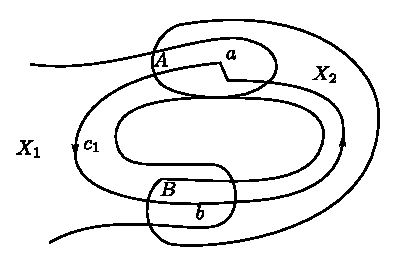
\includegraphics{vol44-fig/fig44-2.eps}
\end{figure}
 
 Let us denote by $\gamma$ a generator of $\mathbb{Z}$ (the infinite
 cyclic group written multiplicatively). By (\ref{thm2.2}) there is a
 unique
 homomorphism $h : \pi (X_1) \ast \mathbb{Z} \to \pi (X)$ such that
 $h(j)= [c]$ and $h | \pi (X_1)$ is induced by the inclusion $X_1
 \subset X$. Now, we have a more precise formulation of (\ref{thm3.1}):  
 \end{proof}

 \medskip
 \noindent
 \textbf{$\boldsymbol{(3.1)'}$. $\boldsymbol{h}$ is an isomorphism}.
 
 Consider\pageoriginale the semi-group of words $W =W (\pi (X_1) \cup 
 \mathbb{Z})$ and the canonical homomorphism $h_c :W \to W /W_0  =
 \pi (X_1) \ast \mathbb{Z}$ where $W_0$ is the equivalence class of
 the empty word. Let us set $\tilde{h} = h\circ h_c : W \to \pi (X)$.  Then,
 $(3.1)'$ is equivalent to:   
 
 \medskip
 \noindent
 \textbf{$\boldsymbol{(3.1)''}$. $\boldsymbol{\tilde{h}}$ is surjective and
   its kernel is $\boldsymbol{W_0}$}. 
 
 For $(3.1)''$ implies that $h$ is an isomorphism. 
 
 Let us say that a path in $X$ is \textit{small}, if it is contained
 in $X_1$ or in $X_2$. For every  point $x \in X$, let $d(x)$ be a
 path such that 
 
if  $x \in B$, $d(x)$ is connecting  $x$  to  $b$  in $B$,  

if  $x \in A$, $d(x)$ is connecting  $x$  to  $a$  in $A$, 
 
if  $x \not\in A \cup B$  and  $x \in X_i$, $d(x)$  is connecting  $x$  to
$a$ in $X_i (i =1 \text{ or } 2)$. Thus, in any case, $d(x)$ is a
small path. Now, let $w$ be a path in $X$ closed at $a$, so that $w$
is an element of $\pi (X)$. If $w \subset X_1$, we  denote by
$[w]_1 \in \pi (X_1)$ its homotopy class in $X_1$. Let $s$ be a
subdivision of $w$ into a product $w = w_1 w_2 , \ldots, w_n$ of small
paths $w_i$. Since $X_1$ and $X_2$ are open, such a subdivision always
exists. We are going to define a well determined word $M(w,s)$
associated to this subdivision of $w$. 

 Let $t_i$ be the terminal point of $w_i$ (and also the initial point
 of  $w_{i +1}$) and $d_i = d(t_i)$ the small path joining $t_i$ to $a$
 or $b$. Let us set 
 $$
 w'_1 = w_1 d_1, w'_i = d^{-1}_{i -1} w_i d_i (i =2, \ldots, n-1), 
 w'_n = d^{-1}_{n-1} w_n ; 
 $$  
 so\pageoriginale that $w'_i$ is a small path contained in the same
 set $X_1$ or $X_2$ as $w_i$, and   
 $$
 w'_1 w'_2 \cdots w'_n = w_1 d_1 d^{-1}_1 w_2 d_2 \cdots d^{-1}_{n-1}
 w_n \thickapprox w. 
 $$

 That will be called \textit{the first modification} of the product. 
 
 Now, we take off those $w'_i$ which are closed and $\thickapprox 0$
 in $X_1$ or in $X_2$, in particular, as $X_2$ is simply connected,
 all $w'_i$ which are closed in $X_2$. If $w'_i$ is connecting $b$ to
 $a$ in $X_2$,  $w'_i \thickapprox c_2$ in $X_2$, $w'_i \approx
 c^{-1}_1 c_1 c_2 = c^{-1}_1 c$ in $X$ and we replace $w'_i$  by
 $c^{-1}_1 c$. If $w'_i$ is connecting $a$ 
 to $b$ in $X_2$, $w'_i \thickapprox c^{-1}_2$ in $X_2$, $w'_i
 \thickapprox c^{-1}_2 c^{-1}_1 c_1 =  c^{-1} c_1$ in $X$ and we
 replace $w'_i$ by $c^{-1} c_1$. Thus we get a product of paths, which
 are either contained in $X_1$ or equal to $c$ or $c^{-1}$, 
 $$
 w  \cdots c^{\pm 1} w''_j \cdots w''_k c^{ \pm 1} w''_1 \cdots. 
 $$ 
 
  That will be called \textit{the second modification}.
 
 It may  happen that all $w'_i$ have been taken off in which case $w
 \thickapprox 0$ and we set $M(w,s)=$ the empty word. 
 
 If that is not the case, we replace every maximal series of consecutive
 paths contained in $X_1$ by their product: $w''_j \cdots w''_k  =
 \bar{w}_\ell$, and we get a product 
 $$
 w \cdots c^{\pm 1} \bar{w}_\ell c^{\pm 1} \cdots
 $$ 
 of paths which are either equal to $c$ or $c^{-1}$ or contained in
 $X_1$ and closed at $a$ (the end points of $\bar{w}_\ell$ must be $a$
 because $c$ is closed at (a). That is  \textit{the third and last
   modification}. 
 
Now\pageoriginale we define $M(w,s)$ as the word we get by replacing,
in this product, every path $\bar{w}_\ell$ contained in $X_1$ by its
homotopy class $[\bar{w}_{l}]_1 \in \pi (X_1)$ in $X_1$, and  $c$
by $\gamma$, $c^{-1}$ by $\gamma^{-1}$:     
$$
 M(w, s) = \cdots \gamma^{\pm 1}[\bar{w}_l]_1 \gamma^{\pm 1} \cdots. 
 $$
 
  We have now the following properties.
 \begin{enumerate}[(a)]
\item $\tilde{h} M(w, s) = [w]$. For, by the definition of
  $\tilde{h}$, we have 
$$
\tilde{h} \gamma = [c], \tilde{h}
  \gamma^{-1} = [c^{-1}], \tilde{h} [\bar{w}_l]_1 = [\bar{w}_l]. 
$$

There follows that $\tilde{h}$ \textit{is surjective}. 

\item \textit{If in the product $w_1 \cdots  w_n$ we replace a small 
  path $w_j$ by another small path $v_j$, such that  $v_j \thickapprox
  w_j$ in $X_1$ or in $X_2$, the associated word $M(w,s)$ does not
  change}. For, after the first modification, $v_j$ will be replaced
  by $v'_j \thickapprox w'_j$ in $X_1$ or in $X_2$, and if $w_j
  \subset X_2$, the product we get after the second modification will
  be the same; if $w_j \subset X_1$, after the third modification one 
  of the paths $\bar{w}_l$ will be replaced by a path $\bar{v}_l
  \thickapprox \bar{w}_l$ in $X_1$ so that $[\bar{v}_l]_1 =
               [\bar{w}_l]_1$ and we get the same word 

\item \textit{If we take off or add, in the product $w_1 \cdots,w_n$,
  a path contained in $A$ and closed at $a$, the associated word does
  not change}. For if $w_i \subset A$ is closed at $a$, $w'_i$ will
  be taken off in the second modification. 

\item \textit{If the subdivision $s'$ of $w$ is obtained from $s$ by
  dividing one of the small paths $w_i$ into two paths,} $w_i  = u_i
  v_i$, then $M(w, s') \sim M(w,s)$. 
  \end{enumerate}  
  
  Here\pageoriginale the proof, though quite easy, is a bit longer. If
  we replace $w_i$ by $u_iv_i$, after the first modification,
  $w'_i$ will be replaced by $u'_i v'_i \thickapprox w'_i$ in $X_1$ or
  in $X_2$. If it is in $X_1$, the only  effect after the third
  modification would 
  be to replace a path $\bar{w}_l$ by another one homotopic to it in
  $X_1$ or, if $w'_i$ is closed and $\thickapprox 0$ in $X_1$ while
  $u'_i$ and $v'_i$ are not, to introduce a new path $\bar{w}_l$
  homotopic to zero in $X_1$, so that $M (w, s') =M(w,s)$. If  $u'_i
  v'_i \thickapprox w'_i$ in $X_2$ and $w'_i$ is connecting  $a$ to
  $b$ or $b$ to $a$, one of the paths $u'_i$ or $v'_i$ will be closed
  and taken off in  the second modification, so that again $M(w,s')=
  M(w,s)$. The same holds, if $w_i  \subset X_2$, $u'_i$ and $v'_i$ are
  all closed. 
  
  If $w'_i  \subset X_2$ is closed at a while $u'_i$ is connecting $a$
  to $b$ in $X_2$ and $v'_l$ $b$ to  $a$ in $X_2$, $w'_i$ will be
  taken off in the second modification while $u'_i  v'_i$ will be
  replaced by $c^{-1} c_1 c^{-1}_1 c$, so that if $e_1$ denotes the
  unit element of $\pi (X_1)$, we have $M(w,s) = M_1 M_2$ and
  $M(w,s')=M_1 \gamma^{-1} e_1 \gamma M_2$, and consequently $M(w,s')
  \sim M(w,s)$. 
  
  If $w'_i \subset X_2$ is closed at $b$ while $u'_i$ is connecting
  $b$ to $a$ and $v'_i$ $a$ to $b$, $w'_i$ will be taken off in the second
  modification, while $u'_i v'_i$ will be replaced by $c^{-1}_1 c
  c^{-1} c_1$. Since it is closed at $b$, it must be preceded and
  followed by paths in $X_1$, so that after the second modification we
  get products like 
  $$
   \ldots w''_k w''_ h \ldots \text{~ and~ } w''_k c^{-1}_1 c c^{-1}c_1
   w''_h \ldots. 
  $$
  
There follows that the path $\bar{w}_i$ coming from $\cdots w''_k
w''_h \cdots$ after the third modification is the product of two paths
$u = \cdots w''_k$ and $v=  w''_h \ldots$, connecting $a$ to $b$ and
$b$ to $a$, $\bar{w_i}= uv$, and will be replaced\pageoriginale by
$\bar{w}_{l_1} cc^{-1} \bar{w}_{l_2}$ with $\bar{w}_{l_1} =
uc^{-1}_1$ and $\bar{w}_{l_2}= c_1 v$. Setting $[\bar{w}_l]_1 = \xi$,
$[\bar{w}_{l_1}]_1 = \xi_1$ and $[\bar{w}_{1_2}]_1 = \xi_2$, we have  
$$
M(w,s) =  M_1 \xi M_2, M(w,s') = M_1 \xi_1 \gamma \gamma^{-1} \xi_2
M_2 
$$ 
and $M(w,s) \sim M(w,s')$ because $\xi= \xi_1\xi_2$.


Hence (d) is proved. An immediate consequence is:
\begin{enumerate}
\item[(e)] \textit{If $s$ and $s'$ are any two subdivisions of $w$ into
  small paths, $M(w,s)\break \sim M (w,s')$}. 

For any two subdivisions have a common refinement, and any refinement
can be obtained by introducing one point at a time. 

\item[(f)] \textit{If $w \thickapprox 0$ in $X$, then $M(w,s)\sim W_o$}
\end{enumerate}

As $\tilde{h}M(w,s) = [w]$, this means that $\ker \tilde{h} = W_o$ and
will achieve the proof of (\ref{thm3.1}). 

The homotopy $w \thickapprox 0$ consists of a map $F: I\times I \to X$
such that $F(I \times 0) = w$, $F(0 \times I) =  F(I \times 1) = F(1
\times I) =a$. Let us divide the square $I \times I = ( 0 \le s, t \le
1)$ into $m^2$ equal squares, $m$ being great enough in order that
their images by $F$ be small in $X$, i.e contained in $X_1$ or in
$X_2$. We number these squares in such a way that the one of centre
$(s,t)$ comes before the one of centre $(s', t') $ if $t < t'$ or
$t=t'$ and $s < s'$. Let $v_j$ be the path, product of $2m$ edges of
our chessboard, connecting $(0,1)$ to $(1,0)$ by passing above the
first $j$ squares and under the other. Here is a representation of
$v_{16}$ with $m=6$. 
\begin{figure}[H]
\centering
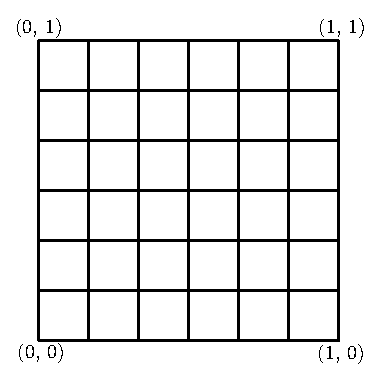
\includegraphics{vol44-fig/fig44-3.eps}
\end{figure}
$F(v_j)$\pageoriginale is a path closed at $a$ and has $a$ subdivision
$s_j$ into $2m$ small paths, the images of the edges of $v_j$. Let us
compare the words $M_{j-1} = M(F(v_{j-1}),  s_{j-1})$ and $M_j=
M(F(V_j), s_j)$. Let $u$, $v$ be the sides of the $j^{\rm th}$ square in
$v_{j-1}$ and $u'$, $v'$ the sides in $v_j$  
\begin{figure}[H]
\centering
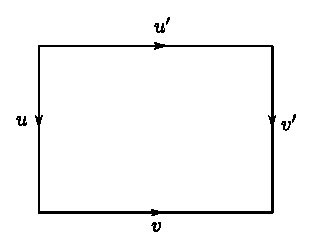
\includegraphics{vol44-fig/fig44-4.eps}
\end{figure}

We get the product $F(v_j)$ from $F(v_{j-1})$ by replacing $F(u)
F(v)$ by $F(u') F(v')$, so that we have 
$$
F(v_{j-1}) = PF (u) F(v) Q, F(v_j) = PF(u') F(v') Q. 
$$

But $F(u) F(v) =F(uv)$ and $F(u') F(v') =F(v' v')$ are small paths,
homotopic in the same set $X_1$ or $X_2$. By (b), the words
associated to\pageoriginale $PF(uv)Q$ and to $PF(u' v')Q$ are the
same, and by (d) they are equivalent to $M_{j-1}$ and $M_j$, so that
$M_{j-1} \sim M_j$. Hence $M_o \sim M_{m^2}$. But, by (c) and (d),
$M_o \sim M (w,s)$, and as $F(v_{m^2}) =a$, $m_{m^2}=$ the empty $w$
so that $M(w,s) \in  W_o$.  

\begin{theorem}\label{thm3.2} %\thm 3.2
Suppose $X = X_1 \cup X_2$ is the union of two arcwise connected
  open sets $X_1$ and $X_2$, whose intersection $X_o = X_1 \cap X_2$,
  is non void and arcwise connected. The groups $\pi (X)$ and $\pi
  (X_i)$ being based at the same point $a \in X_o$, let $j_i: \pi
  (X_o) \to \pi (X_i) \; (i=1,2)$ be the homomorphism induced by the
  inclusion $X_o  \subset X_i$, and  $J$ the set of relations $J = \{
  j_1(\alpha) = j_2 (\alpha), \alpha \in  \pi (X_o) \}$. Then 
$$
\pi (X) \simeq \pi (X_1) \ast \pi (X_2) /J.  
$$
  \end{theorem}  
  
By (\ref{thm2.2}), there is a unique homomorphism $h: \pi (X_1) \ast  \pi
(X_2) \to \pi(X)$ such that $h | \pi (X_i)$ is induced by the
inclusion $X_i \subset X(i =1,2)$. Now, a precise formulation of
(\ref{thm3.2}) is: $(3.2)'$ ~ $h$ \textit{is surjective and has the same kernel
  as the canonical homomorphism of $\pi (X_1) \ast \pi(X_2) $ onto
  $\pi (X_1) \ast \pi (X_2) / J$}. 
  
Consider the semi-group of words $W=W ( \pi (X_1) \cup \pi
(X_2))$, let $W_o$ be the equivalence class of the empty word and $W_J
\supset W_0$ its $J$-equivalence class. Then $W/_{W_J} = \dfrac{\pi
  (X_1) \ast \pi (X_2)}{J}$. Let  $h_c$ be the canonical homomorphism
$h_c : W \to  W_{W_o}= \pi (X_1) \ast \pi (X_2)$, and $\tilde{h} = h
o h_c$. Then $(3.2)'$ is equivalent to \textit{$(3.2)'' \tilde{h}$ is
  surjective and its kernel is $W_J$}. 
  
The\pageoriginale proof of similar to that of $(3.1)''$, but
easier. We say, again, 
that a path is small, if it is contained in $X_1$ or in $X_2$, and for
every $x \in X$, we choose a path $d(x)$ connecting $x$ to $a$, such
that $d(x) \subset X_i$ if $x \in X_i (i= 0,1,2)$. For any path $u$
closed at $a$, we denote by $[u] \in  \pi (X)$ its homotopy class in
$X$ and if $u \subset X_i$, by  $[u]_i \in \pi (X_i)$ its homotopy
class in $X_i$. 
  
Let $w$ be a path closed at $a$ in $X$ and $s$ a subdivision
of $w$ into a product $w = w_1 w_2 \cdots w_n$ of small paths. We are
going to define two words $M^1(w,s)$ and $M^2(w,s)$. We set again $d_i
= d(t_i)$ with $t_i =$ terminal point of $w_i, w'_i = d^{-1}_{i-1}
w_i  d_i \; (i=2, \ldots, n-1)$, $w'_n =  d^{-1}_{n-1} w_n$, and we
get a new product  
  $$
  w'_1 w'_2 \cdots w'_n \thickapprox w 
  $$   
  where $w'_i$ is a small path contained in the same set $X_1$ or
  $X_2$ as $w_i$, and closed at $a$. Now, replacing, in this product,
  $w'_i$ by $[w'_i]_1 \in \pi (X_1)$ if $w'_i \subset X_1$ and by
  $[w'_i]_2 \in 
  \pi (X_2)$ if $w'_i  \not\subset X_1$, we get the word $M^1
  (w,s)$. Similarly, replacing $w'_i$ by $[w'_i]_2 \in \pi (X_2)$ if
  $w'_i \subset X_2$ and by $[w'_i]_1 \in \pi (X_1)$ if $w'_i
  \not\subset X_2$, we get the word $M^2(w,s)$. These two words differ
  only if some $w'_i$ are contained in $X_1 \cap X_2 = X_o$, in  which
  case we have $[w'_i]_1 = j_1 [ w'_i]_o$ in $M^1 (w,s)$ and $[w'_i]_2
  = j_2 [ w'_i]_o$ in $M^2 (w,s)$. As $\tilde{h}[w'_i]_j =[w'_i]
  \in \pi (X)$,  by the definition of $\tilde{h}$, we have, 
  \begin{enumerate}
\item[(a$'$)] \textit{The\pageoriginale two words $M^1 (w,s) $ and
  $M^2(w,s)$ are $J$-equivalent and $\tilde{h} M^1\break (w,s)=  \tilde{h}
  M^2 (w,s) = [w]$}, 

Hence $\tilde{h}$ is \textit{surjective}. We have further the 
following properties. 

\item[(b$'$)] \textit{If, in the product $w = w_1 \cdots w_n$ we
  replace $w_i$ by another small path $v_i$ homotopic to $w_i$ in
  $X_j \; (j =1 \text{ or } 2)$, the word $M^j (w,s)$ does not change}. 

That is immediate because we will have $v'_i \approx w'_i$ in
$X_j$. The following is also immediate. 

\item[(c$'$)] If we take off or add in the product $w_1 \cdots w_n$
  \textit{a small path closed at $a$ and $\approx 0$ in $X_o$, the only
    effect will be to take off or to add in $M^j (w,s)$ a unit
    element}. 

\item[(d$'$)] \textit{If the subdivision $s'$ of $w$ is obtained from
  $s$ by dividing one of the small paths $w_i$ into two parts, $w_i =
  u_i v_i$, and if $w_i \subset X_j  \; (j=1 \text{ or } 2)$, then $M^j
  (w,s')$ is $J$-equivalent to $M^j(w,s)$}. 
  \end{enumerate}

The proof is similar to that of (d) in the former case, but
easier. For $w'_i$ will be replaced by $u'_i v'_i$, $w'_i =
d^{-1}_{i-1} w_i d_i =  d^{-1}_{i-1} (u_i v_i) d_i$ and $u_i v'_i =
d^{-1}_{i -1} u_i dd^{-1} v'_i d_i$, where $d=d$ (terminal point of
$u_i$). As all these paths are in $X_j$,  $w'_i \approx u'_i v'_i$ in
$X_j$ and $[w'_i]_j = [u'_i]_j [v'_i]_j$, we have $M^j(w,s')$ is
$J$-equivalent to $M^j(w,s)$. 

\begin{itemize}
\item[(e$'$)] \textit{If $s$ and $s'$ are any two subdivisions of $w$
  into small paths,\break $M^j(w,s')$ and  $M^j (w,s)$ are $J$-equivalent}. 

\item[(f$'$)] \textit{If\pageoriginale $w \approx 0$ in $X$, then
  $M^j(w,s) \in W_j$}. The proof is the same as that of (c) and
  (f) in the former case, so that $(3.2)''$ is established.  
\end{itemize}
  
  An important corollary is the following.
  
  \begin{theorem}\label{thm3.3}% \thm (3.3)
 The notations and the hypotheses being the same as in (\ref{thm3.2}),
  let $i_1 : \pi (X_o) \to \pi (X_1)$ and $i_2 :  \pi (X_o)  \to
  \pi (X_2)$ be the homomorphisms induced by the inclusions $X_o
  \subset X_1$ and $X_o \subset X_2$: 
\[
\xymatrix{
& \pi (X_1) \ar[dr]^{j_1} \\
\pi (X_0) \ar[ur]^{i_1} \ar[dr]_{i_2} & & \pi (X) \\
& \pi (X_2) \ar[ur]_{j_2} & 
}
\]
 If $i_1$ and $i_2$ are injective, then $j_1$ and $j_2$ are also injective.
  \end{theorem}  
  
That follows from the fact that if $i_1$ and $i_2$ are injective,
$\pi (X) \simeq \pi (X_1) \ast \pi (X_2) /J$ is a free product
with amalgamation. 
  
If in the statements (\ref{thm3.1}) and (\ref{thm3.2}) one replaces
the condition 
that $X_1$ and $X_2$ be open by that they be closed, without changing
the other hypothesis, the  conclusion do not remain valid in general,
as can be shown by counter examples. Nevertheless, for many
applications, the following remark is useful. 

\setcounter{remark}{3}
\begin{remark}\label{rem3.4} % \rem 3.4
If $X =X_1 \cup X_2$ is the union of two closed sets $X_1$ and
 $X_2$, satisfying all other hypotheses of theorem (\ref{thm3.1}) (resp.
 (\ref{thm3.2}) and (\ref{thm3.3}) and if there are open sets $Y_1$
and $Y_2$, such 
 that $Y_1 \supset X_1$, $Y_2 \supset X_2$, $X_i$\pageoriginale is a
 deformation restract of $Y_i \; (i = 1,2)$ and $X_1 \cap X_2$ is a
 deformation retract of $Y_1 \cap Y_2$, then the conclusion of 
 (\ref{thm3.1})-(resp. (\ref{thm3.2}) and (\ref{thm3.3})-remain valid. 
\end{remark}   
   
   For we can apply the theorem (\ref{thm3.1}) to $Y_1$ and $Y_2$ instead of
   $X_1$ and $X_2$, and as $\pi(Y_i) =  \pi(X_i) \; (i  = 1,2
   \text{ or } 0)$ we get the conclusion. 
      
\begin{note*}
 The theorem (\ref{thm3.2}) is usually named van {\em Kampen's} theorem. In
 the case where $X$ is a simplicial complex and $X_1$ and $X_2$ are
 subcomplexes of $X$,  it was first given by Seifert. Van Kampen gave
 a more general theorem which contains both (\ref{thm3.1}) and
 (\ref{thm3.2}).  
\end{note*}   

\section{Examples}\label{sec4} % \sec 4

\medskip
\noindent\textbf{1. The circle {\boldmath$S^1$}.}\pageoriginale

Suppose that $p$ and $q$ are two points on the circle $S^1$. Then $S^1 
- p$ and $S^1 -q$ are both simply connected open subsets of $S^1$ and
their intersection consists of two arcwise connected simply connected
sets. Hence by theorem (\ref{thm3.1}) we have  
\begin{figure}[H]
\centering
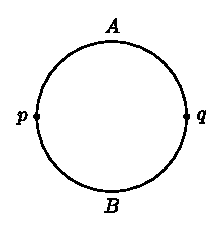
\includegraphics{vol44-fig/fig44-6.eps}
\end{figure}
$$
(S^1) \simeq 1 \ast \mathbb{Z} = \mathbb{Z}.  
$$

\medskip
\noindent{\textbf{2. The sphere {\boldmath$S^n = \{ x=  (x_1, \ldots,
      x_{n+1}),  \sum\limits_{1}^{n+1} x^2_i =1 \}$, $n \ge 2$}.}}  

It follows from (\ref{thm3.2}) that the union of two simply  connected open
sets, whose intersection is arcwise connected, is simply
connected.\break Here, if $p$, $q$ are two distinct points of $S^n$, as $S^n
= (S^n -p) \cup (S^n -q)$ and $(S^n -p) \cap (S^n -q)$ is arcwise
connected for $n \ge 2$, $\pi (S^n)$ is trivial. 

\medskip
\noindent{\textbf{3. The wedge of {\boldmath$n$} circles.}}  We consider
a set of $n$ circles $C_1, C_2, \ldots, C_n$ every two of which
meet at a point $p$. We denote the union of $C_1, \ldots, C_n$ by
$B_n$.  
  
   Let $q$ be a point of $C_n$, $q \neq p$.  $B_{n-1}$ is a
  deformation retract of $B_n -q$, hence (corollary 1.3) $\pi
  (B_{n}-q) = \pi(B_{n-1})$. Now $B_n = (B_n -q) \cup (C_n-p)$,
  while $(B_n -q) \cap (C_n -p) = C_n -p-q$ is the union of two
  disjoint simply connected open sets. Hence, by (\ref{thm3.1}), $\pi (B_n)
  = \pi(B_{n-1}) \ast \mathbb{Z}$, and by induction $\pi (B_n) =
  \mathbb{Z} \ast\cdots \ast  \mathbb{Z}$ ($n$ copies). 
  
  Now\pageoriginale suppose that we take the circles $C_i$ in the
  $(x,y)$ plane as  
  $$
  C_i = \{(x,y) : (x-i)^2 + y^2 = i^2 \}.
  $$
  
  \noindent
  We provide $B_\infty$ with the topology induced from the plane. In
  this topology every compact set in $B$ is contained in some
  $B_n$. Hence if $F$ gives a homotopy between two paths in $B_\infty$
  it does so in some $B_n$. Now using the previous result we obtain 
  $$
  \pi  (B \infty) = \underset{i\in I}{\ast} \mathbb{Z}_i
  $$
  where  $I$ is a countable indexing set.
   
  If we take the circle $( x- \dfrac{1}{n})^2 + y^2 =  \dfrac{1}{n^2}$
  for $C_n$ then the group $\pi(B_\infty)$ is much more complicated
  since, in this case, a path need not be contained in a finite number
  of the $C_i$. 

\medskip
\noindent{\textbf{4. Attaching an {\boldmath$n$}-cell to a space.}}
  
 We denote the coordinate in euclidean $n$-space by $x_1, x_2,
 \ldots, x_n$. We denote the $n$-disc by $D^n$, its boundary the
 $(n-1)$-sphere by $S^{n-1}$ and the $n$-cell by $e^n$: 
\begin{align*}
D^n  & =  \left\{ (x) | x^2_1 + x^2_2 + \cdots +  x^2_n \le 1 \right\} \\
S^{n-1} & = \left\{ (x) |  x^2_1 + x^2_2 +  \cdots + x^2_n = 1 \right\} \\
e^n &= \left\{ (x) | x^2_1 + x^2_2 + \cdots +  x^2_n < 1 \right\} 
\end{align*}   
   
      Suppose that $X$ is a topological space and that $f$ is a map of
      $S^{n-1}$ into\pageoriginale $X$. Then we consider the disjoint
      union $X \cup D^n$ of $X$ and $D^n$ and introduce the
      following relation:  
   $$
   x = y \text{ if } x=y  \text{ or } x= f(y) \text{ or } y = f(x)
   \text{ or } f(x) = f(y). 
   $$
   
   It is clear that this is an equivalence relation and we denote the
   quotient space by $X \cup_f D^n$. We note that the point set
   underlying this space can be identified with $X \cup e^n$ and that
   with this identification $X \cap e^n = \phi$. This process of
   constructing a new space is called attaching an $n$-cell. Now we
   study the effect, on the fundamental group, of attaching an
   $n$-cell. 
   
   We choose an interior point $p$ of $D^n$. We denote the set $X
   \cup_f D^n - p$ by  $X_1$ and $e^n$ by $X_2$. Then since the radial
   projection of $D^n-p$ gives a deformation retraction of the set
   onto $S^{n-1}$ we have that $X$ is a deformation retract of
   $X_1$. Hence 
   $$
   \pi (X_1) \simeq \pi (X).
   $$
   
It is clear that $S^{n-1}$ is a deformation retract of $e^n -p$ and
hence we have   
   $$
   \pi (e^n -p ) \simeq  \pi (S^{n-1}).
   $$
   
   Applying our theorem (\ref{thm3.2}) to $X_1$, $X_2$ we obtain in view of (2) 
   $$
   \pi (X \cup_f D^n) \simeq \pi (X) \text{ if } n \ge 3.
   $$
$\boldsymbol{n=1}$. In this case $e^1 -p$ consists of two connected
   components. We know that $e^1$ is simply connected. Hence applying theorem
   (\ref{thm3.1}) with $X_1= X \cup_f D^1-p$, $X_2 = e^1$ we obtain 
$$
\pi (X \cup_f D^1) \simeq \pi (X) \ast \mathbb{Z}. 
$$
$\boldsymbol{n=2}$.\pageoriginale In this case $e^2-p$ is connected
and $\pi (e^2 -p)$ is generated by a single  element say $a$. We know that
$\pi (e^2) =1$ and hence applying theorem (\ref{thm3.2}) to $X_1 = X \cup_f
D^2 -p$ and $X_2 = e^2$ we obtain 
$$
\pi (X \cup_f D^2) \simeq \frac{\pi (X) \ast 1}{\bar{a} =1} = \pi
(X) /_{\bar{a} =1} 
$$
where $\bar{a}$ is the image of $a$ in $\pi(X_1)$. Since the
boundary of $D^2$ is a deformation retract of $D^2-p$ and a is in
$D^2-p$ it follows that $\bar{a}$ is the class given by the path
$f|S^1$.  

\medskip
\noindent{\textbf{5. Closed surfaces of genus {\boldmath$p$}.}}

Now we give some constructions.

We take a wedge $X$ of $2p$ circles $a_1, a_2,  \ldots, a_p$, $b_1,
b_2, \ldots, b_p$ and a 2-disc $D^2$. We subdivide the circles
$S^1$, boundary of  $D^2$, into $4p$ segments $C_i$. We
homeomorphically map $C_{4i}, C_{4i+1}, C_{4i+2}, C_{4i+3}$ onto
$a_{i+1}, b_{i+1}, a^{-1}_{i+1}, b^{-1}_{i+1}$ in that
order. We denote the resulting map of the $S^1$ by $f$. Then attaching
$D^2$ to $X$ by $f$ we obtain an oriented closed surface of genus
$p$. We denote it by $S_p$. If we denote the generator of $\pi (X)$
corresponding to the circle $a_i$ by $a_i$ itself by (4) above we
obtain  
$$
\pi (S_p) \simeq \{ a_1,  b_1, a_2,b_2, \ldots, a_n, b_n ; a_1, b_1
a_1^{-1} b^{-1}_1 \cdots a^{-1}_n b^{-1}_n =1\}. 
$$

Now we take a wedge $X$ of $p$-circles $a_1, \ldots, a_p$. We
subdivide $S^1$ into $2p$ segments $C_i$. We map $C_{2i}$, $C_{2i+1}$
homeomorphically onto $a_i$, $a_i$, and denote the resulting map of
$S^1$ into $X$ by $f$. Then attaching $D^2$ to $X$ by $f$ we obtain a
non-oriented closed\pageoriginale surface of genus $p$. We denote it
by $S'_p$. If we denote the generator of $\pi(X)$ corresponding to
the circle $a_i$ by $a_i$ itself by (4) we obtain  
$$
\pi (S'_p) \simeq \{ a_1, a_2, \ldots, a_p; a_1 a_1 a_2 a_2 \ldots
a_p a_p = 1 \}. 
$$

Now for any space $X$ we define $H_1(X)$, the first homology group of
$X$, to be the quotient of $\pi(X)$ by the commutator subgroup. It
is clear that the the image of $a_1 b_1 a^{-1}_1 b^{-1}_1 \ldots a_n
b_n a^{-1}_n b^{-1}_n$ in $H_1(S_p)$ reduces to the unit element and
hence $H_1(S_p)$ is a free abelian group with $2p$
generators. Similarly it follows that $H_1({S'}_p)$ is the direct
product of a free abelian group with $(p-1)$ generators and a group of
order 2. Hence it follows that $\pi (S_p)$ and $\pi (S'_q)$ for
various $p$ and $q$ are all distinct. Hence the surfaces we obtain are
pairwise distinct. 

The theorem on the classification of surfaces shows that we thus 
obtain all closed surfaces. 

\medskip
\noindent{\textbf{6. Torus knots.}}

A knot is a simple closed curve in $\mathbb{R}^3$. The fundamental
group of the complement of a knot is called the group of the knot. 
 
We say that two knots are of the same type if there exists an
automorphism of $\mathbb{R}^3$ taking one onto the other. In this case
the corresponding complements in $\mathbb{R}^3$ are homeomorphic and
hence two knots of the same type have the same group. A knot which is
of the type as a circle is called a trivial knot. 

A knot\pageoriginale lying over a torus is called a torus knot.

We take a Cartesian coordinate system $(x, y, z)$ in
$\mathbb{R}^3$. Let $C'$ be the circle  
$$
(y - 10)^2 + z^2 = 1, \quad x = 0; 
$$
or parametrically 
$$
y-10 = \cos \varphi, \quad z = \sin \varphi 
$$
and $T$ be the torus generated by the rotation of $C'$ around the $z$
axis. The parametric equations of $T$ are  
\begin{align*}
x & = (10 + \cos \varphi) \sin \theta\\
y & = (10 + \cos \varphi) \cos \theta\\
z & = \sin \varphi
\end{align*} 
with angular parameters $\varphi$ and $\theta$. We denote the interior
of $T$ by $T^i$ and its exterior by $T^e$. Now let $p$, $q$ be two
positive coprime integers and $C_{p,q}$ the closed curve 
$$
\theta = pt, \varphi = qt,  \quad 0 \leq t \leq 2 \pi.
$$

Since $p$, $q$ are coprime it follows that $C_{p,q}$ is a simple
closed curve. We denote the circle trace by the centre of $C'$ under
the rotation around $0_z$ (the $z$ axis) by $C$. We prove that the
group of this knot is $G_{p, q} = (a, b ; a^p = b^q)$. 

Let $X_1 = \overline{T^i} - C_{p,q}$, $X_2 = \overline{T^e} -
C_{p,q}$. Then $X = 
X_1 \cup X_2 = \mathbb{R}^3 - C_{p,q}$ and $X_1 \cap X_2 = T- C_{p,q}$. Here
$X_1$ and $X_2$ are closed in $X$. Nevertheless, according to the
remark (\ref{rem3.4}), we can apply (\ref{thm3.2}), as there are open sets $Y_1
\supset X_1$ and $Y_2 \supset X_2$ such that $X_1$, $X_2$, $X_1 \cap
X_2$ are\pageoriginale deformation retracts of $Y_1$, $Y_2$ and $Y_1
\cap Y_2$ respectively.  

$\pi (X_1) \simeq \mathbb{Z}$, has as generator the homotopy class
of $C$, and $\pi (X_2) \simeq \mathbb{Z}$ has as generator the
homotopy class of a circle $C''$ concentric with $C'$ with radius
2. Now $T- C_{p,q}$, the torus cut along a closed curve, is
homeomorphic to an annulus and $\pi (T- C_{p,q})= \mathbb{Z}$, with
generator the homotopy class of a curve equidistant of $C_{p,q}$ along
the torus. This curve is homotopic to $C^p$ in $X_1$ and to $C''^q$
in $X_2$. Setting $a = [C]$ and $b= [C'']$, we have by (\ref{thm3.2}) $\pi
C_{p,q} = (a, b; a^p = b^q) G_{p,q}$. 

It follows, by (\ref{sec2.8}), that if $p, q, p', q'$ are integers $>1$
and $(p, q) \neq (p', q') \neq (q, p)$, $C_{p,q}$ and $C_{p',q'}$ are
not of the same type. 

This result was proved by Antoine by a different and highly geometric 
method. 

Now we prove that the knots $C_{p,q}$ and $C_{q,p}$ are of the same
type. For this we compactify $\mathbb{R}^3$ and obtain the 3-sphere 
$$
x^2_1+ x^2_2 + x^2_3 + x^2_4 = 1. 
$$

Now it is easy to see that by means of the transformation 
$$
(x_1, x_2, x_3, x_4) \mapsto (x_3, x_4, x_1, x_2) 
$$
we can obtain $C_{q,p}$ from $C_{p,q}$.


\section{The group of a tame link given by a good plane
  projection}\pageoriginale %% 5

A \textit{link} is a collection of a finite number of pairwise
disjoint knots. We say that two links are of the same type if there
exists an automorphism of $\mathbb{R}^3$ carrying one onto the
other. The fundamental group of the complement of a link is called the
group of the link. 

We say that a link is \textit{tame} if it is of the same type as a
link of polygonal knots, i.e. of knots defined by piecewise linear
simple curves. 

We say that a projection of a link into a plane if \textit{good}, if
the image is a curve with a continuous tangent and a continuous
curvature, whose only singularities are double points with distinct
tangents. The preimage of a double point consists of two points, while
the preimage of any other point of the projection consists of only one
point. 

It can be shown that a link having a good projection is tame and that
any tame link is of the same type as a knot having a good projection
(we are not going to prove this here). We shall now describe a
presentation of the group of a link $C$ given by a good projection. 

Suppose the link lies between the planes $z = -z_0$, $z = z_0$ in the
interior of the cylinder $x^2 + y^2 = r^2$, and has a good projection
into the plane $z = 0$. We choose an orientation on each of its
curves, and take the point $(0, 0, z_0)$ as the base point for the
fundamental group. 

We\pageoriginale denote by $S$ the surface generated by the open half
ray in the direction of negative $z$-axis with end point moving along
$C$  
$$
S= \{ (x,y, z)| \exists \; z' > z \text{ with } (x, y, z') \in C\}
$$
\begin{figure}[H]
\centering
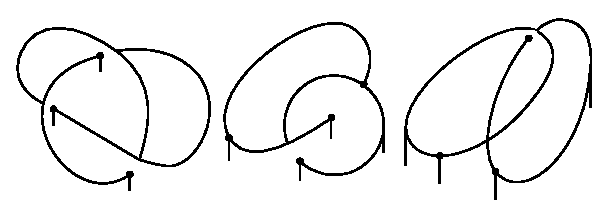
\includegraphics{vol44-fig/fig44-6-1.eps}
\end{figure}

The curves of the link intersect the surface $S$ at points which
divide $C$ into a certain number of arcs. It may happen that a curve
of $C$ does not intersect $S$; in that case we mark a point on it. Now
$C$ is divided by all these points $P_1, \ldots, P_p$ into $p$ arcs
$a_1, \ldots a_p$,  $a_i$ starting from $P_i$. We call them principal
arcs and denote the surface  
$$
 \{ (x,y, z)| \exists \; z' > z \text{ with } (x, y, z') \in a_i \}
$$
by $F'_i$. If a $P_j$ belongs to $F'_i$ then we omit all points of
$F'_i$ lying below $P_j$ including $P_j$ from $F'_i$ and obtain a
surface $F_i$ which is simply connected. We denote the open half ray
through $P_i$ in the direction of the negative $z$-axis by $d_i$. 

To compute the group of $C$ we note that $\mathbb{R}^3 -C$ is obtained by
successive addition of $F_1, \ldots, F_p$ and $d_1, \ldots, S_p$ to
$\mathbb{R}^3 -S$.  

\indent
We set\pageoriginale
$$
D_0 = \mathbb{R}^3 - S, D_i = D_{i -1} \cup F_i \text{ for } i > 1 
$$
and 
$$
E_0 = \mathbb{R}^3- (C \cup D), E_i = E_{i -1} \cup d_i, i>1.  
$$

First let us compare $\pi(D_i)$ and $\pi(D_{i-1})$. Since $C$ has
a good projection it is easy to construct a simply connected set
$F''_i$ such that $D_i \supset F''_i \supset F_i$ and such that $F''_i
\cap D_{i-1}$ consists of two simply connected sets. Hence by (\ref{thm3.1})
we have 
$$
\pi (D_i) = \pi (D_{i-1}) \ast \mathbb{Z}.
$$

We denote the element of $\pi(D_i)$ corresponding to the generator
of $\mathbb{Z}$ and represented by a path crossing $S$ only at one
point from the left to the right by $a_i$ itself. Now we note that
$\mathbb{R}^3 -S$ is simply connected. Hence  
$$
\pi (E_i) = \mathbb{Z} \ast \ldots \ast \mathbb{Z} \; (p \text{ times}). 
$$

Now let us compare $\pi (E_i)$ and $\pi (E_{i-1})$. Since $C$ has a
good projection we can construct an open simply connected
neighbourhood $U_i$ of $d_i$ contained in $E_i$ such that $\pi (U_i -
d_i)$ is infinite cyclic and $E_{i-1} \cap U_i = U_i - d_i$ is
connected. 

In\pageoriginale the case where the projection of $d_i$ is a double
point, crossed by the projection of $a_k$ and separating the
projection of $a_j$ and $a_i$ a generator of $\pi(U_i - d_i)$ in
$E_{i -1}$ is represented by $a_j a_k a^{-1}_i a^{-1}_k$ and the
relation given is $a_j a_k = a_k a_i$ (see figure).  

In the case where the projection of $d_i$ is not a double point and
corresponds to a point marked on a curve which does not cross $S$, a
generator of $\pi (U_i - d_i)$ is represented by $a_i a^{-1}_i$ (see
figure). 

\begin{figure}[H]
\centering
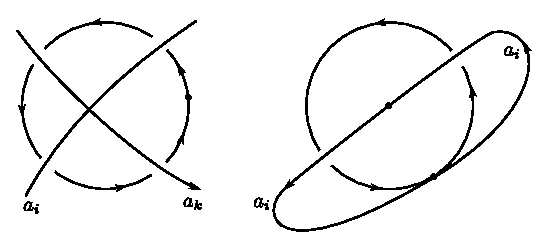
\includegraphics{vol44-fig/fig44-7.eps}
\end{figure}

\noindent
Now by (\ref{thm3.2}) we have 
\begin{align*}
\pi(E_i) & = \pi (E_{i-1}) / \left\{a_i a_k a^{-1}_j a^{-1}_k = 1 \right\}\\
 & = \pi (E_{i-1})  / (a_i a_k = a_k a_j)
\end{align*}
in the first case and 
$$
\pi (E_{i}) = \pi (E_{i-1}) 
$$
it the second.

Now, we show that $\pi (E_{p-1}) \simeq \pi (E_{p})$.

For\pageoriginale we have $E_{p-1} = \mathbb{R}^3 - (C U d_p)$ and $E_p =
\mathbb{R}^3 - C$, and it is easy to see that a small path around
$d_p$ is $\approx 0$ in $E_{p-1}$. Hence  
$$
\pi (E_{p-1}) \simeq \pi (E_{p}).
$$
 
\begin{theorem*}
Let $C$ be a link with a good projection, To every principal arc $a_i$
of $C$ is associated an element of $\pi(\mathbb{R}^3 -C)$ denoted by
the same letter $a_i$ and represented by a path which crosses the
cylinder $S$ in only one point, under $a_i$, from the left to the
right. To every double point of the projection is associated a
relation described in the figure. The elements $a_i$ generate
$\pi(\mathbb{R}^3 -C)$ and these relations form a complete set of
relations, moreover, any one of them is a consequence of all the
others. 
\end{theorem*}

\section{Antoine's Necklace}\label{sec6} % section 6

We\pageoriginale consider a solid torus $T$ and $2p$ solid torus $T_1,
\ldots, T_{2p}$, situated in the interior of $T$ as in the figure.  
\begin{figure}[H]
\centering
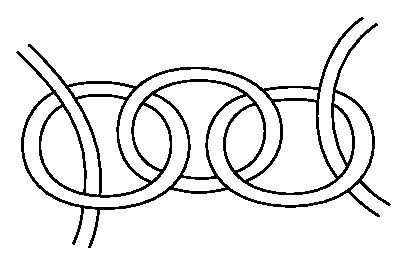
\includegraphics{vol44-fig/fig44-8.eps}
\end{figure}

$T_i$ is linked with $T_{i +1}$, all $T_i$ are congruent to $T_1$ and
similar to $T$, and a rotation through an angle of $2 \pi /p$ around
the axis of $T$ carries $T_i$ onto $T_{i + 2}$. (We take $i({\rm mod}
2p)$). The union $N_1 = \bigcup\limits^{2p}_{i = 1} T_i$ forms an
elementary necklace. 

Let $h_j$ be a similarity of $\mathbb{R}^3$, i.e. a contraction
followed by an isometry, taking $T$ onto $T_j$. Then by means of the
$h_j$ we get $(2p)^2$ tori $h_j T_i$ of second order and, more
generally, we get $(2p)^n$ tori 
$$
h_{ji} \circ  \ldots \circ  h_{j_{n}} T
$$
which we call the tori of order $n$. Their union  
$$
N_n = \bigcup\limits^{1 \ldots 2p}_{j_1 \ldots j_n} h_{j_{1}} \circ 
\ldots \circ  h_{j_{n}} T 
$$
will\pageoriginale be called a necklace of order $n$. The intersection
$$
A = \bigcap^{\infty}_1 N_n
$$
is a perfect totally discontinuous set, discovered and studied by
Antoine, which is called Antoine's Necklace. 

We will show that $\pi (\mathbb{R}^3 -A)$ \textit{is not trivial, even
  not finitely generated.} 

First, \textit{we prove that a meridian of $T$ represents an element
  of infinite order in $\pi(\mathbb{R}^3 - N_1)$.} 
 
If $C$ is the link consisting of the $2p$ circles $c_i\;(i = 1, \ldots,
2p)$ where $c_i$ is the locus of the centres of the meridians of
$T_i$, $\mathbb{R}^3 -N_1$ is a deformation retract of
$\mathbb{R}^3-C$, we have $\pi(\mathbb{R}^3 -N_1) =
\pi(\mathbb{R}^3-C)$. Now, $\pi(\mathbb{R}^3 -C)$ has 4p generators
$a_i, b_i, c_i, d_i(i ({\rm mod} p))$, corresponding to the principal
arcs of $C$ as in the figure, with the relations  
\begin{gather*}
(1) ~~ a_i b_{i -1} = d_{i- 1} a_i, \quad (2) ~~ a_i b_i = d_i a_i,\\
(3) ~~ c_i b_i = b_i a_i \qquad (4) ~~ c_i b_{i-1} = b_{i-1} a_i.
\end{gather*}
\begin{figure}[H]
\centering
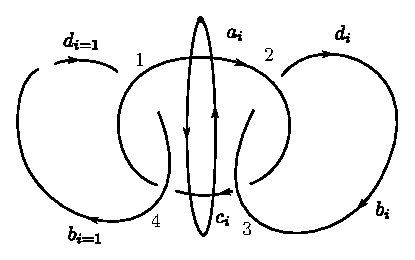
\includegraphics{vol44-fig/fig44-9.eps}
\end{figure}


Now\pageoriginale a meridian $X$ of $T$ represents the element $X= a_i
c^{-1}_i$. There is a homomorphism of $\pi (\mathbb{R}^3 -C)$ onto the
free group of rank two with generators a and $b$, under which the
images of $a_i$, $b_i$, $c_i$, $d_i$ are respectively $a$, $b$,
$bab^{-1}$ and $aba^{-1}$ for every $i$. The image of $X$ being
$aba^{-1} b^{-1}$, an element of infinite order, $X$ is also of
infinite order. As $X$ represents a generator of the infinite cyclic
group $\pi(\mathbb{R}^3 -\overset{o}{T})$, there follows that \textit{the
  homomorphism $\pi (\mathbb{R}^3 - \overset{o}{T}) \to \pi (\mathbb{R}^3 -N_1)$
  induced by inclusion is injective.} 

Now, if we write $D= T = \overset{o}{N_1}$, we have  
$$
T- A = \bigcup^{\infty}_{n=0} \bigcup^{1 \ldots 2p}_{j_1 \ldots j_n}
h_{j_{1}} \circ  \ldots \circ  h_{j_{n}} D. 
$$

\noindent
Let us number the series $(j_1 \ldots j_n)$, taking in succession
those for which $n= 0$, $1, 2, \ldots$, and if $m = m (j_1, \ldots,
j_n)$ is the number of $(j_1, \ldots, j_n)$ let us set $h_{j_{1}} \circ
\ldots \circ h_{j_{n}} D= D_m$, (where $D_0 = D$, $D_1 = h_1 D= T_1 - h_1
N_1, \ldots)$. Then we have  
$$
T- A= \bigcup^{\infty}_{k=0} D_k 
$$
and we set 
$$
E_m = \bigcup^m_{k=0} D_k \cup (\mathbb{R}^3 -T). 
$$

\noindent
We have $D_m \cap E_{m-1} = h_{j_{1}} \circ, \ldots \circ h_{j_{n}} (T -
\overset{o}{T})$, and $E_{m-1}$ is a deformation retract of a set open
in $E_m$. 

Now, we will prove that the inclusion homomorphisms$ \pi (E_{m-1}) \to
\pi(E_m)$ and $\pi(D_m) \to \pi (E_m)$ are injective. If we
set\pageoriginale $X_1 = 
E_{m-1}$, $X_2 = D_m$, we have $X_1 \cap X_2 = X_0 = h_{j_{1}} \circ
\ldots \circ h_{j_{n}} (T - \overset{\circ}{T})$ and $X_1 \cap X_2 =
E_m$. From theorem (\ref{thm3.3}) and remark (\ref{rem3.4}), 
we have only to show that the inclusion homomorphisms  
$$
i_1 : \pi(X_0) \to \pi(X_1) \text{ and } i_2 : \pi(X_0) \to \pi(X_2) 
$$
are injective.

$X_0$ is the surface of the torus $T' = h_{j_{1}} \circ \ldots \circ h_{j_{n}}
T$ and $\pi(X_0)$ is a free abelian group with two generators
represented by a meridian $M$ and a parallel $P$ of that surface. If
$M^a P^b \approx 0$ in $E_{m-1}$, then $M^a P^b \approx M^a \approx 0$
in $\mathbb{R}^3 - \overset{\circ}{T'}$ because $P \approx 0$ in
$\mathbb{R}^3 - \overset{\circ}{T'}$ and $E_{m - 1}
\subset \mathbb{R}^3 - \overset{\circ}{T'}$. This implies $a= 0$. Then
$M^a P^b = P^b \approx 0$ in $E_{m-1}$ implies $b = 0$, because $P$ is
linked with a following torus or the elementary necklace contained in
it, in the same way as $X$ was linked with $T$ or $N_1$. Hence $i_1$
is injective. Similarly one sees that $i_2$ is injective.

Thus the following inclusion homomorphisms 
$$
\pi(\mathbb{R}^3 - T^0 ) \to \pi(E_1) \ldots \pi(E_{m-1}) \to \pi(E_m) 
\ldots 
$$
are injective, consequently $\pi (\mathbb{R}^3 - T) \to \pi
(\mathbb{R}^3 -A)$ is also injective, because if a path in
$\mathbb{R}^3 - A $ is $\approx 0$ in $\mathbb{R}^3 -A$, it is
contained and $\approx 0$ in $E_m$ for $m$ great enough. A meridian of
$T$ is not $\approx 0$ in $\mathbb{R}^3 - A$, and the same is true for
a meridian of any torus of any order $q$. If $q$ is great enough, such
a meridian is not homotopic to a path contained in $E_{m}$, and it
follows that $\pi(\mathbb{R}^3 - A)$ is not finitely generated. 

\medskip
\noindent\textbf{Antoine's horned sphere.}

We\pageoriginale take a solid truncated cone $H_0$ with base in the
plane $z = 0$ 
and the top in $z = 1$. We erect on its top $2p$ congruent disjoint
truncated cones $H_i (i= 1, \ldots, 2p)$ with tops in the plan $z =
2$. We assume the union $H_0 \cup H_1 \cup \ldots \cup H_{2p} = H$ is
a solid bounded by a disk $D$ in the plane $z =0$, the base of $H_0$,
and a surface $z = f(x, y)$, which contains $2p$ discs $D'_i \; (i = 1
\ldots 2p)$ in the plane $z =2$, the top of the $H_i$. 
\begin{figure}[H]
\centering
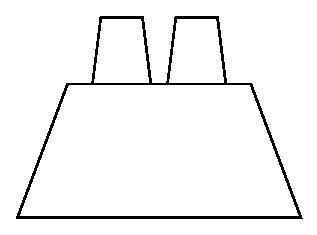
\includegraphics{vol44-fig/fig44-10.eps}
\end{figure}

Now, let $h_i$ by a similarity consisting of a contraction followed by
a translation which takes the base of $H_0$ onto the top of $H_i$. Now
let us set  
$$ 
B = \bigcup^{\infty}_{n=0} \bigcup^{1 \ldots 2p}_{i_1 \ldots i_n}
h_{i_{1}} \circ\ldots \circ h_{i_{n}} H. 
$$

The closure $\bar{B}$ of $B$ is a 3-disk, bounded by the base of $H$
and a surface $z = g(x, y)$, where $g(x,y)$ is continuous in the base
of $H$ and zero on its boundary. Moreover, $0 \leq g(x, y) \leq
\dfrac{2}{1-r}$, where $r$ is the ratio of the similarities $h_i$. The
set $\bar{B} \cap \{ z = \dfrac{2}{1-r}\}$ is a perfect totality
discontinuous set $A'$ on the boundary of $\bar{B}$. 

Now, let us consider a 2-disk $D$ on the boundary of $T$ and its image
$h_i D = D_i$ on the boundary of $T_i \; (i = 1, \ldots, 2p)$. One can
find a homeomorphism $f$ of $H$ into $T - N^\circ_1$, such that $fD' = D$,
$fD'_i = D_i$ and $f \circ h'_i (x) = h_i \circ f(x)$ for any $x \in D'$ This
homeomorphism has a unique extension from $H$ to $\bar{B}$ satisfying
$f \circ h'_i (x) = h_i f(x)$\pageoriginale for any $x \in \bar{B}$. Then
$f(\bar{B})$ is a 3-disk contained in $T$, whose boundary contains
$A$. For $A$ is the image under $f$ of the set $\bar{B} \cap \{ z =
2/1 -r \}$, the top of $\bar{B}$. Hence, a closed path linked with $T$
in $R^3 -T$ is not $\approx 0$ in $R^3 - f(\bar{B})$, and we see
that \textit{the complement $R^3 - f(\bar{B})$ of the 3-disc
  $f(\bar{B})$, is not simply connected.}  

Antoine proved, more generally, that for any compact totally
discontinuous set $A$ in $\mathbb{R}^n$, there is an imbedding $f :
D^n \to \mathbb{R}^n$ such that $f(S^{n-1}) \supset A$. 

\section{Elementary ideals-Alexander polynomials}\label{sec7}%%% sec 7

In\pageoriginale the last section we have seen how to get a
presentation of the group of a link. It is often quite difficult to
decide, from presentations, whether two groups are distinct. In this
section, we give some invariants of a group that can be calculated
easily from a presentation.  

Suppose that $A$ is a commutative ring with a unit element 1 and
that $M$ is a finitely generated $A$-module. Then we associate to $M$
a finite sequence of ideals of $A$ called elementary ideals. If $M_1$
is an $A$-module and $M_2$ is a submodule of $M_1$ then the values $m
(M_2)$ taken over $M_2$ of linear forms $m$ on $M_1$ generate an ideal
which we denote by $\mathfrak{a} (M_1, M_2)$. Now we take a finite system $s
= [ \alpha_1, \ldots, \alpha_n]$ of generators of $M$ and consider the
free module $U = A^n$ with the natural basis $u_1, \ldots, u_n$. We
denote the homomorphism of $U$ onto $M$ taking $u_1$ onto $\alpha_i$
by $h$ and denote the kernel of $h $ by $V$. We define the ideals
$\mathfrak{a}_p(s)$ by setting  
$$
\mathfrak{a}_p (S) =  
\begin{cases}
 \mathfrak{a} (\overset{P}{\Lambda} U, \overset{P}{\Lambda} V) & p \geq 1,\\
(1) = A, & p \leq 0.
\end{cases}
$$

We have $\mathfrak{a}_p (s) \supset \mathfrak{a}_{p +1} (s)$. Now we proceed to
show that this sequence of ideals essentially depends only on $M$. For
this we examine $\mathfrak{a}(U, V)$ more closely. The linear forms on $U$
are generated by $u^*_i (i = 1, \ldots, n)$ where $u^*_i$ is the linear
form defined by  
$$
u^\ast_i (u_j)= 
\begin{cases}
& 1 \text{ if } i = j\\
& 0 \text{ if } i \neq j.
\end{cases}
$$
$u^\ast_i (m)$\pageoriginale is precisely the $i$-th component of
$m$. Hence $\mathfrak{a} (U, V)$ is the ideal generated by the components of
elements in $V$. To study the relation between $a_p (s)$ and $a_p
(s')$ where $s'$ is another system of generators of $M$ we start with
$s' = [\alpha_1, \ldots, \alpha_n, \alpha_{n+1}]$. Since $s$ generates
$M$ we have  
$$
\alpha_{n+1} = \sum^n_{j=1} C_j \alpha_j
$$
for some elements $C_j$ of the ring $A$. We take the natural basis
$u_1, u_2, \ldots,\break u_n, u_{n+1}$ of $A^{n+1} = U'$ and set 
$$
h' (u_i)= 
\begin{cases}
& \alpha_i \text{ for } i  \leq n,\\
& \alpha_{n +1}\text{ for  } i = n+ 1.
\end{cases}
$$

 
We denote the kernel of $h'$ by $V'$. To compute $\mathfrak{a}(U', V')$ we
change the basis of $U'$ so that the elements of $V'$ can be obtained
easily from those of $V$. The new basis consists of $u_1, u_2, \ldots,
u_n$ and $u = u_{n+1} - \sum\limits^n_{i=1} c_i u_i$. Then $h'(u) =
\alpha_{n+1}-\sum \limits^n_{i=1} c_i \alpha_i = 0 $. And hence an
element $\sum\limits^n_{i=1} b_i u_i + bu$ of $U'$ belongs to $V'$ if
and only if $\sum\limits^n_{i=1} b_i u_i$ belongs to $V$. So $V' = V
\oplus A_u$ and  
$$
\mathfrak{a}_{p+1} (s') = \mathfrak{a}_p (s). 
$$

Now, let $s_1$ and $s_2$ be any two systems of $n_1$ and $n_2$
generators. Then $s = s_1 \cup s_2$ is a system of $n_1 + n_2$
generators and it follows from the above that $\mathfrak{a}_{r +1} (s) =
\mathfrak{a}_{r} (s_1)$, $\mathfrak{a}_{r +n_1}(s) = \mathfrak{a}_{r}(s_2)$. 

Consequently\pageoriginale  
$$
\mathfrak{a}_{r + n_{1}} (s_2) = \mathfrak{a}_{r +n_{2}}(s_1). 
$$
Let us denote the last non-zero ideal $\mathfrak{a}_{p}(s)$ in the sequence
$\mathfrak{a}_{i}(s)$, where $s$ is any system of generators, by
$\mathfrak{a}_{p}(s) = A_1 (M)$ and set  
$$
A_i (M) = \mathfrak{a}_{p-i +1}(s) \; (i = 1, 2, \ldots.)
$$
Form the above relation it follows that this sequence $A_i (M)$
depends only on $M$. These ideals are called the \textit{elementary
  ideals of $M$}. We have $A_i(M) \subset A_{i +1} (M)$ and $A_i (M)
= A$ for $i$ great enough. 

Suppose that $V$ is generated by the elements  
$$
v_i = \sum^n_{j=1} a_{ij} u_j \quad (i= 1, 2, \ldots, m).
$$
Then, for the definition, it follows that $\mathfrak{a} (\Lambda U, \Lambda
V)$ is the ideal generated by the minors of order $p$ in the matrix
$(a_{ij})$ and is zero if $p> n$ or $p > m$. 

Now let us take a knot group $G = (a_1, \ldots, a_p; R_1, \ldots,
R_q)$. Let us denote $[G, G]$ by $G'$ and $[G', G']$ by $G''$ and the
images of $a_i$ in $G/G'$ by $\bar{a}_i$. Since it is a knot group, $G/
G'$ is the infinite cyclic group. We denote its group ring by $A$ and
denote a generator of $G/G'$ by $x$, the other one being $x^{-1}$. We
have  
$$
A = \mathbb{Z}[x, x^{-1}], 
$$
the polynomial ring of two variables $X$, $Y$ quotiented by the ideal
$(XY-1)$. 

Let\pageoriginale us show now that $G' / G''$ is an $A$-module, and is
finitely generated. If $t \in G$ has $x$ as canonical image in $G/ G'$,
$x = tG'$, and if $\alpha \in G' / G''$, the automorphism of $G'
/G''$ defined by $\alpha \to t \alpha t^{-1}$ depends only on 
$x$. Hence to $x$ is associated a well determined automorphism of $G'
/ G''$ and each element of $A$ represents a well-determined
endomorphism of $G' / G''$, so that $G' / G''$ is an $A$-module. 

Suppose further that $a_1, \ldots, a_n$ generate $G$. Let $x^{n_{i}}$
be the canonical image of $a_i$ in $G / G'$; then $a_i t^{-n_{i}} 
\in G'$ and the elements $t$,  $a_1^{t^{-n1}}, \ldots, a_n^{t^{-nn}}$
generate $G$. Now, the elements $t^k ( a_i t^{-n_{i}}) \;  t^{-k} (i =
1, \ldots, n$; $k= 0$, $\pm 1$, $\pm 2, \ldots)$ generate $G'$. Let
$\alpha_i$ be the canonical image of $a_i t^{-n_i}$ in $G' / G''$. There
follows that $\alpha_1, \ldots, \alpha_n$ generate $G' / G''$ as an
$A$-module. Moreover, the relations of the presentation of $G$ give a
set of relations defining this $A$-module. 

Every element $\neq 0$ of $\mathbb{Z} [x, x^{-1}]$ can be written
uniquely in the form  
$$
\pm x^k P(x), 
$$
where $P(x) \in \mathbb{Z}[x]$ is such that $P(0) > 0$. We say that
$P(x)$ is a normalized polynomial. The units of $\mathbb{Z} [ x,
  x^{-1}]$ are the elements $\pm x^k \; (k \in \mathbb{Z})$. As
$\mathbb{Z} [x]$ is a unique factorization domain, there follows that
any set of elements of $A$ (containing at least one element $\neq 0$)
has a greatest common divisor, (i.e. an element which divides all
these elements and is divided by each of their common divisors,)
represented by a well determined normalized polynomial. 

In\pageoriginale particular, the elements of the ideal $A_i (G' /
G'')$ have as a greatest common divisor a normalized polynomial $A_i
(x)$. These are called the \textit{Alexander polynomials} of the
knot. $A_i (x)$ is divisible by $A_{i+1} (x)$, and $A_i (x)= 1$ for
$i$ great enough. The most interesting is the first $A_1 (x)$, also
denoted by $A (x)$. Form our definition, there follows that these
polynomials are well determined by the group $G$ of the knot and the
choice of a generator $x$ of $G/G'$. By taking the other generator
$x^{-1}$ instead of $x$, one would get a second series of
polynomials. But it can be shown that the elementary ideals are
invariant by the conjugation $x \mapsto x^{-1}$ in $\mathbb{Z}[x,
  x^{-1}]$ and that the Alexander polynomials are reciprocal. Hence
the two series are identical (we shall not prove it here. But this will
be verified in the examples), and \textit{if two knots are of the
  same type, they have the same chain of elementary ideals and the
  same Alexander polynomials.}   

Now we compute the Alexander polynomial and elementary ideals of some
knots. 

First we remark that if a group $G$ is given by a presentation $\{a_i
: R_j \}$ then $G/ [G,G]$ is given by $\{a_i ; R_j, a_k a_\ell =
a_\ell a_k \}$. 
\begin{enumerate}[1)]
\item \textbf{Trefoil knot.}

\begin{figure}[H]
\centering
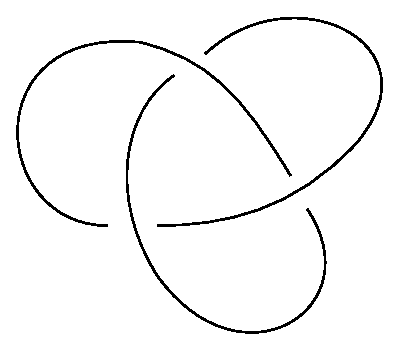
\includegraphics{vol44-fig/fig44-11.eps}
\end{figure}

The group $G$ is given by the presentation 
$$
G= \{ a, b, c; ba= ac = cb \}. 
$$

If\pageoriginale we set $\alpha = ac^{-1 }$, $\beta = bc^{-1}$ then we
obtain  
\begin{align*}
& G = \left\{ c, \alpha, \beta; \beta c  \alpha c = \alpha c^2 = c
  \beta c \right\} \\
\text{or  } \qquad & c, \; , \; ; \beta c \alpha c^{-1} = \alpha = c
\beta c^{-1}
\end{align*}

Denoting the generator of $G/ G'$ corresponding to $c$ by $x$ and
passing to the additive notation and replacing $c \alpha c^{-1}$ by $x
\alpha$, $c \beta c^{-1}$ by $x \beta$, we have the following
relations: 
\begin{align*}
 (x-1) \alpha + \beta & = 0 \; ({\rm mod} G'') \\
 -\alpha + \beta & = 0 \; ({\rm mod} G'').
\end{align*} 
Hence 
$$
A(x) = x^2 - x + 1. 
$$
and the second elementary ideal is (1).


\item \textbf{Torus knot of type {\boldmath$(p, q)$}.}
\end{enumerate} 

We have $G = (a, b; a^p = b^q)$, $(p,q) =1$. We suppose that $p > 1$,
$q> 1$, $p < q$, and that $p'$, $q'$ are such that $pq' - p' q = 1$,
$p' > 0$, $q' > 0$. Now set $t = a^{-p'} b^{q'}$. Then we have  
\begin{align*}
a = a^{pq' - p' q} & = (a^{-p'})^q (b^{q'})^q.\\
& \equiv (a^{-p'}b^{q'})^q  ({\rm mod}   G')\\
& \equiv t^q ~({\rm mod}   G')\\
and \qquad & \equiv t^p   ({\rm mod}   G'). 
\end{align*}

Now let elements $\alpha$, $\beta$ be defined by the equations
$$
a = \alpha t^q, b= \beta t^p. 
$$

From the paragraphs above, it follows that $\alpha$, $\beta$ together
with their\pageoriginale conjugates with respect to $t$ and its powers
generate $G'$. We have $\alpha = at^{-q}$, $\beta = bt^{-p}$ and the
relations $a^p = b^q$ and $a^{p'} t = b^q$. The first gives  
\begin{align*}
 & \alpha t^q \alpha t^q \cdots \alpha t^q = \beta t^p \cdots \beta t^p \\
\text{i.e. }  \qquad \qquad  & t^q t^{-q} t^{2q} t^{-2q} t^{3q}  = t^p
t^{-p} t^{2p}\ldots. \qquad \qquad  
\end{align*}
Hence, passing to the additive notation, replacing $t^n \alpha t^{-n}$
by $x^n \alpha$ and $t^n \beta t^{-n}$ by $x^n \beta$, we have 
{\fontsize{10pt}{12pt}\selectfont
\begin{gather*}
(1 + x^q+x^{2q}+ \cdots + x^{(p-1)}q) \alpha = (1 + x^p+
  x^{2p}+ \cdots + x^{(q-1)}p) \; \beta \; ({\rm mod} \; G'') \\
\text{i.e. } \qquad 
\frac{(x^{pq}-1)}{(x^q -1)} \alpha - \frac{(x^{pq}-1)}{(x^p -1)} \beta
=0 \; ({\rm mod} \; G''). 
\end{gather*}}\relax


Similarly from the other we obtain
$$
\frac{(x^{p' q}-1)}{(x^q -1)} \alpha - \frac{(x^{q'p} -1)}{(x^p -1)} 
\beta =0 \; ({\rm mod} \;  G'').  
$$
Hence 
$$
A(x) = \frac{(x^{pq} -1) (x^{p'q} -x^{q'p})}{(x^p -1)(x^q -1)} \text{
  and the second ideal is (1) }. 
$$
For many other examples, see \textit{Crowel and Fox: Introduction to
  the Knet Theory} (Ginn and Company, 1963). 


\section{Construction of 3-manifolds}\label{sec8}% sec 8

\medskip
\noindent
\textbf{(a) Whitehead Manifold.}\pageoriginale

Suppose that $T$ is a solid torus and solid torus $T'$ is situated in
the interior of $T$ as shown in the figure. 
\begin{figure}[H]
\centering
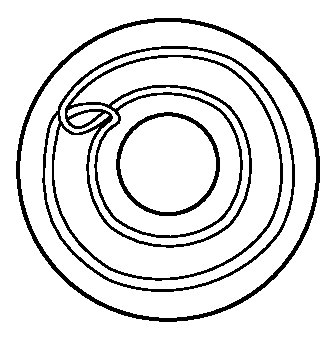
\includegraphics{vol44-fig/fig44-12.eps}
\end{figure}

There exists a homeomorphism $h$ of $\mathbb{R}^3 + (\infty) = S^3$
which fixes points outside a compact set of $\mathbb{R}^3$ and which
takes $T$ onto $T'$. We set 
\begin{align*}
T^{(n)} & = h(T^{(n-1)}) = h^n (T)\\
T^{\infty} & = \bigcap_{n=0}^{\infty} \text{ and } W = S^3 -
T^{\infty}. 
\end{align*}
We note that $T^{(n)} \subset T^{(n-1)}$ and $W$ is a manifold. We
know that $S^3 - \overset{\circ}{T}$ is a torus $T_0$. We set 
$$
T_n = h^n (T_0).
$$
Then\pageoriginale we have 
$$
T_{n-1} \subset T_n \text{ and } W = \bigcup_{n=0}^{\infty} T_n. 
$$
Hence $W$ is the union of an increasing sequence of solid tori. It
has the following properties: 
\begin{enumerate}[(1)]
\item $W$ is simply connected.

\item $W$ is not homeomorphic to $\mathbb{R}^3$

\item $W \times \mathbb{R}$ is homeomorphic to $\mathbb{R}^4$.
\end{enumerate}
We prove the first two of these and only sketch a proof of the third. 

(1) Suppose that $m$ is the meridian of $T$. Then $m$ is homotopic to
the null path in $T_1 = S^3 = \overset{\circ}{T'}$. First it is clear that
$S^3 = \overset{\circ}{T'}$ is a deformation retract of $S^3 - C_1$ where
$C_1$ is the locus of the center of $D^2$ in a representation of $T'$
as $S^1 \times D^2$. 
\begin{figure}[H]
\centering
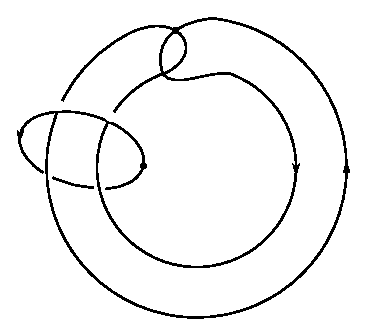
\includegraphics{vol44-fig/fig44-13.eps}
\end{figure}

With the notation of the figure we have  
\begin{align*}
\pi (T_1) &= \{ a,b; a^2 = ba \} \\
[m] & = a^{-1} b
\end{align*}
and hence $m \approx 1$. 

It is clear that the homotopy class of every
closed path in $S^3 - \overset{\circ}{T}$ is a power of $[m]$ and hence it
follows that every closed path in $T_0$ is homotopic to the null path
in $T_1$. By induction it follows that every path in $T_n$ is
homotopic to the null path in $T_{n+1}$. Since every path in $W$ has to
be contained in some $T_n$ it follows that $W$ is simply connected. 

(2) In $\mathbb{R}^3$\pageoriginale every compact set is contained in a
compact set whose complement is simply connected. We prove that the
compact set $T_0$ of $W$ is not contained in a compact set of $W$
whose complement is simply connected. If not there exists a compact
set $K \subset W$ 
and hence $K \subset T_n$ for some $n$ such that $W \supset T_o$ and
$W - K$ is simply connected. Then the meridian of $T^{(n+1)}$ is
homotopic to the null path in $W - K$ and hence in $W- T_0 \subset T -
T^{\infty}$. We prove that this is not the case. 

Let $C_1$ be the image of the circle $S^1 \times 0$ by a homeomorphism
of $S^1 \times D^2$ onto $T'$ and $C_2$ a circle in $\mathbb{R}^3 - T$
bounding a 2-disk which cuts $T$ along a meridian. Then it is clear
that $T - \overset{\circ}{T'}$ is a deformation retract of $S^3 - C_1 -
C_2$ and hence  
$$
G = \pi (T - T') \simeq \pi (S^3 - C_1 - C_2) \simeq \pi (\mathbb{R}^3
- C_1- C_2) 
$$
is isomorphic to the group of the link $C_1 \cup C_2$, given as in the
figure. 
\begin{figure}[H]
\centering
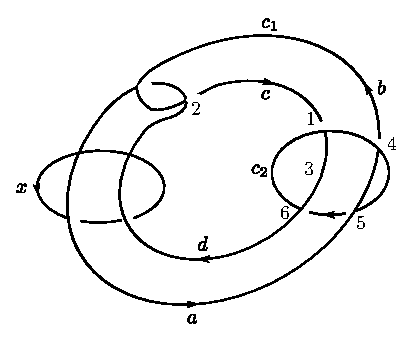
\includegraphics{vol44-fig/fig44-14.eps}
\end{figure}


Then\pageoriginale the homotopy class of a meridian of $T$ is given by
$X$. With the notation of the figure the group $G$ is given by
generators $a, b, c, d, e, f$ and the following relations:

\smallskip
\noindent
(1) $db = ba$, \quad  (2) $bd = dc$, \quad (3) $ed = ce$

\noindent
(4) $ea = be $  \quad (5) $ae = fa$, \quad  (6) $fd = de$.
\smallskip

Since one relation is a consequence of the others we can drop (6) and
eliminate $f$ by means of (5). We are thus left with generators $a,
b, c, d, e$ and relations 1,2,3,4. From (4) we have $a= e^{-1}
be$, and from (1) $d = bab^{-1}$. Eliminating $c$ from (2) and (3) we
obtain 
\begin{gather*}
d^{-1} bd = c = ede^{-1},\\
\text{ i.e. } \qquad be^{-1} b^{-1} ede^{-1}beb^{-1} = ede^{-1}
beb^{-1} e^{-1}. 
  \end{gather*}  
Hence the group is given by the presentation
$$
G =\{ e, b; eb^{-1} e^{-1} be^{-1} b^{-1} ebe^{-1} beb^{-1} ebe^{-1}
b^{-1} = 1 \}. 
$$
In this $X$ is represented by the element
$$
a^{-1} d = e^{-1} b^{-1} ebe^{-1} beb^{-1}. 
$$
Now we prove that this element is of infinite order in $G$. For this
consider the map of $b$ and $e$ into $\mathbb{Z}_2 \ast \mathbb{Z}_2 =
(\alpha, \beta, \alpha ^2 = \beta^2 = 1)$ defined by 
$$
b \mapsto \beta, e \mapsto \beta \alpha. 
$$
Substituting these values in the relator we obtain the word
$$
\beta \alpha \beta \alpha \beta\beta \alpha \beta\beta\beta \alpha
\beta \alpha \beta\beta\beta \alpha \beta\beta \alpha \beta \alpha
\beta\beta 
$$
Since $\alpha^2 = \beta^2 =1$ this becomes the empty word. Hence
the above map can be extended into a homomorphism of $G$ into
$\mathbb{Z}_2 \ast \mathbb{Z}_{2}$. 

Under\pageoriginale this $[X]$ goes into
$$
\alpha \beta\beta\beta \alpha \beta \alpha \beta\beta\beta \alpha
\beta = (\alpha \beta)^4 
$$ 
The word $\alpha \beta$ is reduced and it follows that $\alpha \beta$
and hence $[X]$ is of infinite order. 

Now we can prove that the inclusion homomorphism $\pi (S) \to \pi (T -
\overset{\circ}{T}')$, where $S = T - \overset{\circ}{T}$, is
injective. Denoting the  parallel of $T$ by $Y$, if $X^a Y^b \approx
0$ in $T - \overset{\circ}{T'}$, then we have $X^a Y^b \approx 0$ in $T$
and hence $Y^b \approx 0$ in $T$. This implies that $b = 0$. Then the
result above gives $a = 0$. 

Denoting the boundary of $T'$  by $S'$ one can prove, in a similar
manner, that the inclusion homomorphism  
$$
\pi (S') \to \pi (T - \overset{\circ}{T'})
$$
is injective. But we prefer to indicate a way of obtaining an
involution of $T -\overset{\circ}{T'}$ permuting the boundaries $S'$ and
$S$. The  following sequence of figures gives an involution of $S^3 -
C_1 - C_2$ exchanging $C_1$ and $C_2$. Since $T - \overset{\circ}{T'}$ is
a deformation retract of $S^3 - C_1 - C_2$ we get the result.
\begin{figure}[H]
\centering
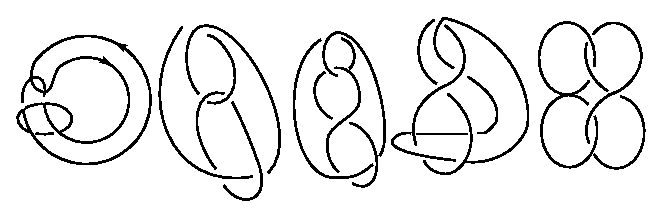
\includegraphics{vol44-fig/fig44-15.eps}
\end{figure}

 Thus the inclusion homomorphism 
$$
\pi (S') \to \pi (T- \overset{\circ}{T'})
$$
is injective.

Using\pageoriginale (\ref{thm3.3}) and induction on $n$ we can show that the
conclusion homomorphism   
$$
\pi (h^n (S)) \to \pi (T -\overset{\circ}{T}^{(n)})
$$
is injective. From this fact and the fact that the inclusion 
homomorphism  
$$
\pi (h^n(S)) \to \pi (T^{(n)} - \overset{\circ}{T}^{(n+1)})  
$$
is injective by (\ref{thm3.3}) it follows that the inclusion homomorphism 
$$
\pi (T- \overset{\circ}{T}^{(n)}) \to \pi (T -
\overset{\circ}{T}^{(n+1)}) 
$$
is injective.

Hence the meridian of $T^{(n)}$ cannot be homotopic to the null path in
$T^{(n)} - T^{\infty}$ and (2) is proved. 

(3) We have seen that
$$
W = \bigcup_{n} T_n, \; T_n \subset T_{n+1} 
$$
where each $T_n$ is a torus. Hence 
$$
W \times \mathbb{R} = \bigcup_n T_n \times I_n 
$$
where $I_n$ is the interval $[-n, n]$. 

Now let $g$ be a homothety which changes the $t$ hours $T''$ into a torus
$g(T'')$, such that there is a sphere in $g(T'')$ containing $T''$. 
\begin{figure}[H]
\centering
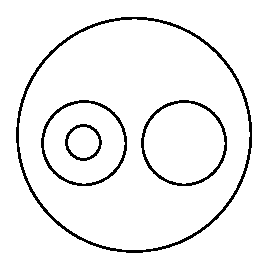
\includegraphics{vol44-fig/fig44-16.eps}
\end{figure}

Let\pageoriginale $T''_n = g(T'')$. It is clear that
$\bigcup\limits_{0}^{\infty} T''_n = \mathbb{R}^4$. 

Now, it can be shown that there exists homeomorphisms $\varphi_n :
T_n \times I_n \to T''_n \times I_n$ such that $\varphi_{n+1}$ is an
extension of $\varphi_n$, because one can unknot $T_n \times I_n$ in
$T_{n+1} \times I_{n+1}$. [See T. Glimm, Bull. Soc. Math France, 1962,
  p] 

\medskip
\noindent
\textbf{(b) Homology 3-spheres of Dehn.}

Now we proceed to give a method, due to Dehn, of constructing homology
3-spheres (i.e. a compact closed manifold $M$ such that $H_{\ast} (M) =
H_{\ast} (S^3)$.), with a fundamental group $G$ identical to its
commutator subgroup $G'$. For this we take a tubular neighbourhood of
a trefoil knot. Then we remove its interior from $S^3$ and attach a
torus to this with a twist. 
\begin{figure}[H]
\centering
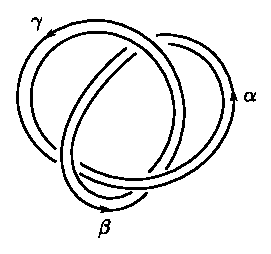
\includegraphics{vol44-fig/fig44-17.eps}
\end{figure}
 
 Let $T$ be a tubular neighbourhood of a trefoil knot. Let the
 notation be as in the figure and let 0 be the base point. We have  
 $$
 \pi (S^3 -\overset{\circ}{T}) = (a, b, c; ad = bc = ca);
 $$
 where\pageoriginale $a, b, c$ are the generators corresponding to
 the principal arcs of the trefoil. Setting $ab = bc = ca = \sigma$
 we have   
 \begin{gather*}
b = a^{-1} \sigma, c = \sigma a^{-1}\\
\sigma = bc = a^{-1} \sigma^2 a, \text{ i.e. } \sigma^2 = a \sigma a.
 \end{gather*} 

Hence $ \pi (S^3 - \overset{\circ}{T}) = (a, \sigma ; \sigma^2 = a \sigma
a)$. 

We have $\sigma a \sigma a = \sigma \sigma^2 = \sigma^2 \sigma = a
\sigma a \sigma $, 
$$
\sigma^3 a = a \sigma a \sigma a = a \sigma^3, 
$$
and hence $\sigma^3$ is in the centre.

$T$ is homeomorphic to a solid torus and the fundamental group of the
surface $S = T - \overset{circ}{T}$, based at the same point 0, is
generated by the homotopy classes $[m]$ and [1] of a meridian $m$
and a ``parallel'' $\ell$, whose homotopy classes in $S^3 - \overset{\circ}{T}$
are a and $c^{-1} a^{-1} b^{-1}$. It is of course also generated by
$[m]$ and $[lm^k]$, for any integer $k$. The homotopy class of $lm^3$ 
in $S^3 - \overset{\circ}{T}$ is  $\lambda = c^{-1} a^{-1} b^{-1} a^3$. As
$c^{-1} a^{-1} b^{-1} = a \sigma^{-1} a^{-1} \sigma^{-1} a$, we have 
$$
\lambda = a \sigma^{-1} a^{-1} \sigma^{-1} a^4 = a (\sigma^{-1} a^{-1}
\sigma^{-1} a^{-1}) a^5 = a \sigma^{-3} a^5 = \sigma^{-3} a^6. 
$$

Let $T'$ be a solid torus and let $h$ be a homeomorphism of $S' = T' -
\overset{\circ}{T'}$ onto $S$, under which a parallel and a meridian of
$S'$ go into curves of $S$ of homotopy classes $\lambda$ and $a
\lambda^{-k}$, where $k$ any integer. We set 
$$
V_k = (S^3 - \overset{\circ}{T}) \bigcup_h T'.
$$
(Using\pageoriginale (\ref{thm3.2}), since the meridian of $S'$ is homotopic to
the null path in $T'$ and $\pi (T')$ is generated by the homotopy
class of a parallel of $S'$, we see that $\pi (V_k)$ is the quotient
of $\pi (S^3 -\overset{\circ}{T})$ by the relation $a \lambda^{-k} = 1$ or
$a \sigma^{3k}  a^{-6k}=1$ or $\sigma^{3k} = a^{6k-1}$, and we get the
presentation  
$$ 
\pi (V_k) = (a, \sigma ; \sigma^2 = a \sigma a, \sigma^{3k} = a^{6k 
  -1}). 
$$
It is clear that the quotient of this group by its commutator subgroup
is trivial. Hence it follows that $H_1 (V_k) = 0$ and that $V_k$ is a
homology 3-sphere. When $k = 0$ we have the 3-sphere, and when $k \neq
0$ we show that $G_k = \pi (V_k)$ is not trivial. In fact $G_k$ and
$G_{k'}$ are not isomorphic if $k \neq k'$. 

For this we examine the representations of $G_k$ into the group of
motions of the non-euclidean plane. In this latter group every
element different from the identity belongs to a unique one-parameter
subgroup which is its normaliser and which consists of all the motions
with the same fixed points. If the representation is non-trivial then
the images $A$ and $S$ of $a$ and $\sigma$ are such that $A \neq 1$,
$S^3 = 1$. For $A = 1$ implies that $S = 1$. Further if $S^3 \neq 1$
then $AS^3 = S^3 A$ gives that $A$ and $S^3$ have the same fixed
points. Hence $A, S$ belong to the same one parameter subgroup and
hence $AS = SA$\pageoriginale which implies $A$ and hence $S$ is
1. This is a contradiction. Hence  
$$
S^3 = (AS)^2 = A^{6k -1} = 1. 
$$
and every representations of $G_k$ comes from a representation of
$G'_k = (A,S; S^3 = (AS)^2 = A^{6k -1} =1)$. 

Now we will show that there exists a faithful representation of $G'_k$
into the group of motions of the non euclidean plane (except if $k
=1$, in which case $G'_1$ is the ikosaeder group $A_5$), and that
$6k-1$ is the maximum order of the elements of finite order. This will
imply the nonisomorphy of $G_k$ and $G_{k'}$ for $k \neq k'$. 

More generally, let us consider the group
\begin{equation*}
G(l,m,n) = \{ A,B; A^l = B^m = (AB)^n = 1 \} \tag{1}\label{eq1}
 \end{equation*} 
 where $l, m, n$ are positive integers. Or, what is the same,
 $$
 G(l,m,n) = \{ A,B,C; A^l = B^m = C^n = ABC = 1 \}.
 $$ 
 Clearly, $G'_k = G(1,2,3)$ with $l = 6k -1$ if $k > 0$ and $l = 1-6k$ if
 $k < 0$. 
 
 Let $s = \dfrac{1}{l} + \dfrac{1}{m} + \dfrac{1}{n}$. We suppose $s <
 1$ and we will construct a faithful representation of $G(l, m, n)$
 into the group of the\pageoriginale motions of take non euclidean
 plane (for $s = 
 1$ or $s > 1$, one would have to take the euclidean plane or the
 sphere and there is a similar construction). 
 
 Let $\Delta$ be a triangle in the non euclidean plane with vertices
 $A', B', C'$ and angles $\alpha = \dfrac{\pi}{l}$, $\beta =
 \dfrac{\pi}{m}$, $\gamma = \dfrac{\pi}{n}$. Let us denote by $a,
 b, c$ the symmetries of the (non euclidean) plane with  respect to
 the sides $B' C'$, $C' A'$, $A' B'$ of $\Delta$ in that order. Then
 $A= bc$, $B = ca$ and $C = ab$ are rotations around $A', B'$ and
 $C'$ of angles $2\alpha$, $2\beta$ and $2\gamma$ respectively, and we
 have 
 $$
 A^l = B^m = C^n = ABC = 1. 
 $$
 The group  $G$ generated by $A$, $B$ and $C$ gives a representation
 of $G(l,m,n)$. 
 
 We will show that this representation is faithful. For this, it will
 be sufficient to show that if a product $X_1 X_2 \ldots X_n$, where
 $X_i$ is an element of the set $E = \{ A, B, A^{-1}, B^{-1} \}$, is
 the identity element of $G$, then the word $X_1 X_2 \ldots X_n$ is
 equivalent to the empty word under the relations given in \eqref{eq1}.  
 
 The quadrilateral $Q = \Delta \cup c (\Delta)$, union of $\Delta$ and
 its  reflection $c(\Delta)$, has as vertices $A', B', C'$ and
 $c(C')$. It is adjacent to its four images $XQ (X, \in E)$
 i. e. images by $A, A^{-1}$, $B, B^{-1}$. Take the
 \textit{disjoint} union $M$ of its images $g(Q)$ by all $g \in
 G$. There is a natural projection of $M$ into the plane. Then, for
 any $g \in G$ and\pageoriginale $X \in E$, let us identify the
 points of $g(Q)$ 
 and $gX(Q)$ which have the same projection (they are the points of
 the side along which $g(Q)$ and $gX(Q)$ are adjacent). After all
 these identifications, we get from $M$ a surface $\tilde{M}$ and a
 natural projection $p$ of $\tilde{M}$ into the plane. It is easy to
 see that $p$ is a covering map, and since the plane is simply
 connected and $M$ is connected, that $\tilde{M}$ is the same as the
 plane. Without reference to the theory of covering maps, it means
 that one has only to show that if $w(t) \; (0 \leq t \leq 1)$ is a path
 in the plane and $x_o \in \tilde{M}$ such that $p(x_o) = w(0)$, there
 is a unique path $\tilde{w} (t)$ in $\tilde{M}$ such that $\tilde{w}
 (0) = x_0$ and $p \tilde{w} (t) = w(t)$, and if $w_s (t)\; (0 \leq s
 \leq 1)$ is a homotopy in the plane, with $w_o (t) = w(t)$, there is
 a unique homotopy $\tilde{w}_s (t)$ in $\tilde{M}$ such that
 $\tilde{w}_0 (t) = w(t)$ and $p \tilde{w}_s (t) = w_s (t)$. This
 means that \textit{the quadrilaterals $g(Q)$ cover the plane and do 
   not overlap}. 
 
 Now, we consider a path $w$ closed at a point $q \in  \overset{\circ}{Q}$,
 which does not pass through any vertex of any quadrilateral $g(Q)$ and
 meets the sides of the $g(Q)$ only in a finite number of simple
 crossings. Such a path $w$ goes through a series of quadrilaterals 
 $$
Q, X_1 (Q), X_1 X_2 (Q), \ldots, X_1 X_2 \ldots X_{n-1}(Q), X_1, X_2
\ldots X_n (Q) = Q, 
 $$  
 where $X_i \in E$ and $X_1 X_2 \ldots X_n =1$. We will say that the
 path $w$ and  the word $X_1 X_2 \ldots X_n$ are associated. Clearly,
 for each such word, representing the unit element of $G$, one can find
 such that a path associated to it. 
 
 If\pageoriginale $w$ is contained in the star $A'$ i.e. the star with
 centre $A'$, i.e. in the union $\bigcup\limits_{i=0}^{l-1} A^k (Q)$
 of the $g(Q)$ such that $A' \in g(Q)$, then $X_i = A$ or $A^{-1}$ for
 each $i$ and 
 it is easy to  see that the associated word $X_1 X_2 \ldots X_n$ is
 equivalent to the empty word on account of the relation $A^l =
 1$. There is a similar result if $w$ is contained in the star
 $\bigcup\limits_{k=0}^{m-1} B^k(Q)$ with centre $B'$ or in the star
 $\bigcup\limits_{k=0}^{n-1} (AB)^k \; (Q \cup A(Q))$ with centre $C'$. 
 
 Now, let us take any word $T = X_1 X_2 \ldots X_n$ representing the
 unit element of $G$, and let $w$ be an associated path. As $w$ is
 homotopic to zero, by the method used in \S \ref{sec3}, one can find a series
 of paths $w_i (i = 0, 1, 2, \ldots, N)$ associated to words $T_i$,
 such that $w_o = w$, $w_N \subset \overset{\circ}{Q}$ and $w_i$ differs
 from $w_{i-1}$ only in the image by some $g \in G$ of a star $S$ of
 centre $A'$, $B'$ or $C'$. That means that $w_i$ and $w_{i-1}$ are
 products like $w_i = u_1 u_2 u_3 $, $w_{i-1} = u_1 u'_2 u_3$, where
 $u_2$ and $u'_2$ are contained in the image of the same star $S$.
 There follows that $T_i$ and $T_{i-1}$ are products of the form $T_i
 = U_1 U_2 U_3$, $T_{i-1} = U_1 U'_2 U_3$, and $U'_2 U^{-1}_2$ is
 associated to the path $U^{-1}_1 \left((u'_2 u^{-1}_2) \right)$; the image by
 $U^{-1}_1$ of the path $u'_2 u^{-1}_2$, which is contained in the
 star $S$. By the remark above, $U'_2 U^{-1}_2$ is equivalent to the
 empty word (on account of the relations \eqref{eq1}), there follows that
 $U'_2$ is equivalent to $U_2$, $T_{i-1}$ is equivalent to $T_i$ and
 $T = T_0$ is equivalent to $T_N$ which is the empty word because $w_N
 \subset \overset{\circ}{Q}$. 

 
 By this, we have proved that $G$ is a faithful representation of\break $G 
 (l,m,n)$. 
 
 Now,\pageoriginale let us consider an element of finite order of
 $G$. In the plane 
 (non - euclidean like euclidean), any motion of finite order is a
 rotation and leaves a point fixed. For an element of $G$, this point
 is necessarily a vertex of some quadrilateral $g(Q)$ and there follows
 that it is conjugate to a power of $A, B$ or $C$. Hence its order
 is a divisor of $l, m, n$.  
 
 That is all what  we needed to prove the non isomorphy of $G_{k'}$
 for $k \neq k'$. 

\section[Involutions of $S^4$.....]{Involutions of $S^4$. Four
  dimensional contractible 
  manifolds whose boundaries are not simply connected. One parameter
  group of homeomor-\break phisms of $S^5$}\label{sec9}\pageoriginale % section 9  

Let us fix some notations. $\mathbb{R}^{n-1}$ shall be considered as a
subspace of $\mathbb{R}^{n}$ defined by $x_n = 0$ and we shall denote
the half spaces $x_n \geq 0$ and $x_n \leq 0$ bounded by
$\mathbb{R}^{n-1}$ in $\mathbb{R}^{n}$ by $\mathbb{R}^{n}_+$ and
$\mathbb{R}^{n}_-$. We shall always suppose that $\mathbb{R}^{n}$ is
compactified with a point at infinity which allows us to identify it
with $S^n$.  

Let us consider a tubular neighbourhood $T_+$ of a simple arc joining
two points of $\mathbb{R}^{2}$ in $\mathbb{R}^{3}$ and knotted as a
trefoil knot (Figure 1). We shall suppose that $T_+$ is bounded by two
circular discs in $\mathbb{R}^{2}$ and a differentiable surface lying
orthogonally on the circles which bound the above discs in such a
manner that the union of $T_+$ with its reflection $T_-$ with respect to
$\mathbb{R}^{2}$ is a solid torus $T= T_+ \cup T_-$ homeomorphic, even
diffeomorphic to the product $D^2 \times S^1 $ (Figure 1) 
\begin{figure}[H]
\centering
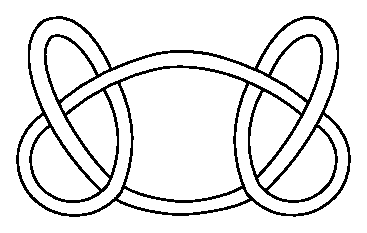
\includegraphics{vol44-fig/fig44-18.eps}
\end{figure}


 By\pageoriginale taking the unit disc $|z| \leq 1$ in the complex
 number plane for 
 $D^2$ and by denoting the angular variable on $S^1$ by $\theta$, the
 points of $T$ are described, thanks to the above homeomorphism of $T$
 and $D^2 \times S^1$, by $(z, \theta)$. We can suppose that $-
 \dfrac{\pi}{2} \leq \theta \leq \dfrac{\pi}{2}$ in $T_+$ and the
 points $(z, \theta)$ and $(z, \pm \pi - \theta)$ are symmetric with
 respect to $\mathbb{R}^{2}$. Let us call the arc described by $(z,
 \theta)$, where $\theta$ varies from $- \dfrac{\pi}{2}$ to
 $\dfrac{\pi}{2}$ as $z$ is kept fixed, \textit{fibre of} $T_+$. The
 union of this arc with its reflection with respect to $\mathbb{R}^{2}$ is a
 simple, closed, differentiable curve $z \times S^1$ which we
 \textit{shall call a fibre of} $T$. 
 
 By rotating $T_+$ around $\mathbb{R}^{2}$ in $\mathbb{R}^{4}$ we
 generate a four dimensional manifold $A$. Each fibre of $T_+$
 generates an $S^2$ which we shall call a fibre of $A$. Let $(z,
 \theta, \psi)$ be a point of a $A$ which is obtained from the point
 $(z, \theta)$ of $T_+$ by a rotation through an angle $\psi$ around
 $\mathbb{R}^{2}$ and $s = s(\theta, \psi)$ be  the point on the
 standard sphere $S^2$ with latitude $\theta$ and longitude $\psi$.
 To each pair $(z,s)$, $z \in D^2$, $s \in S^2$ corresponds a point of
 $A$ and conversely. Thus  we may write $A = D^2 \times S^2$.  
 
 The symmetry with respect to $\mathbb{R}^{3}$ changes the point
 $(z,s)$ of $A$ into the point $(z,s')$ where $s' = s (\theta, \psi)$
 and $s' = s(\theta, - \psi)$ are symmetric on $S^2$ relative to the
 plane containing the meridian $\psi = 0$ and $\psi = \pm \pi$. These
 two meridians together form the great circle $S^1$ of $S^2$ and one
 has  
 $$
 A \cap \mathbb{R}^{3} = T_+ \cup T_- = T = D^2 \times S^1.
 $$
 Each\pageoriginale fibre of $A$ intersects $\mathbb{R}^{3}$ in a fibre of
 $T$. Denoting the boundary $\partial D^2$ of $D^2$ by $S^1_0$ we have 
 $$
  \partial A = S^1_0 \times S^2, \partial A \cap \mathbb{R}^{3} = 
  \partial T = S^1_0 \times S^1.  
 $$
 Now let us consider the two varieties $A$ and $B = \mathbb{R}^{4} -
 \overset{\circ}{A}$, whose union id $\mathbb{R}^{4}$ and whose 
 intersection is their boundary $\partial A = \partial B$, as two
 disjoint manifolds and let $h : \partial A\to \partial B$ be a
 homeomorphism compatible with the symmetry relative to
 $\mathbb{R}^{3}$, i.e. which changes two points of $\partial A$
 symmetric relative to $\mathbb{R}^{3}$ into symmetric points. By
 attaching $A$ to $B$ with the homeomorphism $h$ we obtain a four
 dimensional manifold $V(h) = A \bigcup\limits_{h} B$ which admits an
 involution $J$ which restricted to $A$ as well as to $B$ reduces to
 the symmetry  relative to $\mathbb{R}^{3}$. The set of fixed points
 of this involution is a three dimensional manifold $M(h)$ which we
 obtain by attaching $A \cap \mathbb{R}^{3} = T$ to $B \cap
 \mathbb{R}^{3} = \mathbb{R}^{3} - \overset{\circ}{T}$ by the
 homeomorphism $h$ restricted to $\partial A \cap \mathbb{R}^{3} =
 \partial T$. If $h$ is a diffeomorphism one can define a differentiable
 structure on $V(h)$ and $M(h)$ in a natural way and the involution
 $J$ will then ve a diffeomorphism.
 
 Let $r_{\varphi}$ be the rotation of $S^2$ through an angle $\varphi$
 around the diameter perpendicular to the plane containing the great
 circle $S^1$. If $s$ and $s'$ are symmetric relative to this plane
 $r_\varphi (s)$ and $r_{\varphi} (s')$ are also
 symmetric. Consequently the homeomorphism   
$$
g: \partial A \to \partial A
$$
defined by setting 
$$
g(e^{i \varphi}, s)  = (e^{i \varphi }, r_{\varphi} (s))
$$
is\pageoriginale compatible with the symmetry relative to
$\mathbb{R}^{3}$. Now we have the following proposition.  

\setcounter{proposition}{0}
\begin{proposition}\label{prop1}%proposition 1
Whatever be to the homeomorphism $h : \partial A \to \partial B$
  compatible with the symmetry relative to $\mathbb{R}^{3}$, the
  manifolds $V(h\circ g^2) $ and $V(h)$ are homeomorphic. 
\end{proposition}

\begin{proof}
One knows that $S0 (3)$, the group of rotations of $S^2$ is
homeomorphic to the real projective space of three dimensions and that
its fundamental group is cyclic of order 2. It follows that the map
of $S^1_0$ into $S0(3)$ which sends $e^{i \varphi}$ to $r_{2 \varphi}$
is homotopic to a constant map (This fact, however, can be easily
verified directly). Consequently one can find a continuous, even
differentiable map of $S^1_0 \times I$ into $S0 (3)$, $(e^{i \varphi},
t) \to r_{2 \varphi, t} \; (t \in I = [0,1])$ such that 
$$ 
r_{2 \varphi, 1} = r_{2 \varphi} \text{ and } r_{2 \varphi, t} =
\text{ identity for } t \leq \frac{1}{2}.  
$$ 

Then by setting
$$
f(te^{i \varphi}, s) = (te^{i \varphi}, r_{2 \varphi, t}(s)) 
$$
we can define a homeomorphism, even diffeomorphism 
$$
f : A \to A
$$
which extends $g^2$ to the interior of $A$. Finally we define a
homeomorphism 
$$
F : V(h\circ g^2) \to V(h) 
$$
by $F | A = f$ and $F|B =$ identity. Since the pair of points of $a
\in \partial A$, $b = h\circ g^2 (a) \in \partial B$ which are
identified in $V(h\circ g^2)$ is changed\pageoriginale by $F$ into the
pair of points 
$f(a) = g^2 (a)$ and $b = h\circ g^2 (a)$ which are identified in $V(h)$
the map $F$ is well defined. 

Let us remark that this method does not prove that $V(h ~ \circ~ g)$ and
$V(h)$ are homeomorphic since the map of $S'_\circ$ into $S0(3)$ which
takes $e^{i \varphi}$ to $r_{\varphi}$ is not homotopic to a constant
map (see Addendum). 

It is evident that if one takes for $h$ the identity then $V(h) =
\mathbb{R}^{4}$ and $M(h) = \mathbb{R}^{3}$, $J$ then reducing to
symmetry relative to $\mathbb{R}^{3}$. By composing the identity with
a power $g^k$ of $g$  one obtains manifolds $V_k = V(g^k)$ and $M_k =
M(g^k)$. Then from proposition \ref{prop1} it follows that $V_{2k}$ \textit{is
  homeomorphic to $\mathbb{R}^{4}$ (i.e. $S^4$) and even diffeomorphic
  to it and that the involution $J$ provides a differentiable
  involution $J_{2k}$ of $S^4$ whose fixed point set is $M_{2k}$}. 

The interest in this arises from the following proposition whose proof
shall be given later. 
\end{proof}

\begin{proposition}\label{prop2}%proposition 2
The fundamental groups $G_k = \pi (M_k)$ of the manifolds $M_k$ for $k
= 0, 1, 2, \ldots$ are pairwise non-isomorphic. 
\end{proposition}

Consequently the manifolds $M_k$ are pairwise non-homeomorphic  and
thus we have infinitely many differentiable involutions $J_{2k}$ of
$S^4$ which are distinct. 

It follows from the proposition \ref{prop1} that $V_{2k +1}$ is homeomorphic
to $S^4$ (see Addendum). 

The\pageoriginale manifold $V_{2k} = S^4$  is partitioned by $M_{2k}$
into two 
manifolds $V^+ _{2k}$ and $V^-_{2k}$ which are permuted by the
involution $J_{2k}$. We obtain $V^+ _{2k}$ by attaching $A_+ = A \cap
\mathbb{R}^{4}_+$ to $B_+  = B \cap \mathbb{R}^4_+$ with the
homeomorphism $g^{2k}$ restricted to 
$\partial A \cap \mathbb{R}^{4}_+$. The sphere $S^2$ is partitioned by
$S^1$ into two half- spheres $S_+^2$ and $S_-^2$ and each
fibre $z \times S^2$ of $A$ is partitioned by the $z \times S^1$ of $T$
into two half-spheres $z \times S^2_+ \subset A_+$ and $z \times S^2_-
\subset A_-$.  

By rotating $\mathbb{R}^{4}_+$ around $\mathbb{R}^{3}$,
$\mathbb{R}^{5}$ is generated and is partitioned by $\mathbb{R}^{4}$
into $\mathbb{R}^{5}_+$ and $\mathbb{R}^{5}_-$. Every half sphere $z
\times S^2_+$ generates a three dimensional sphere $z \times S^3$
which is  partitioned by $z \times S^2$ into two half- spheres $z
\times S^3_+$ and $z \times S^3_-$ and $A_+$ generates a five
dimensional manifold $A$ fibred by the spheres $z \times S^3$ and
partitioned by $A$ into $\tilde{A}_+$ and $\tilde{A}_-$. We see that
$\tilde{A}_+$ is  obtained, in a way, from $A$ by replacing the fibers
of $A$, which are two dimensional spheres $z \times S^2$ by the three
dimensional half spheres $z \times S^3_+$. Thus  
\begin{align*}
\tilde{A} &= D^2 \times S^3 \qquad, \tilde{A}_+ = D^2 \times S^3_+\\
\partial \tilde{A} & = S_o^1 \times S^3 \qquad, \partial \tilde{A}_+
= (S^1_0 \times S^3_+) \cap A. 
\end{align*}
Likewise $B_+$ generates the manifold $\tilde{B}$ which is partitioned
by $B$ into $\tilde{B}_+$ and $\tilde{B}_-$. Every rotation $r$ of
$S^2$ extends in a natural way into a rotation $\tilde{r}$ of $S^3$
which preserves $S_+^3$ and $S_-^3$. Consequently the homeomorphism $g
: \partial A \to \partial A$ where $\partial A = S^1_0
\times S^2$ and $g (e^{i \varphi}, s) = (e^{i \varphi}, r_{\varphi}
(s))$ extends to a homeomorphism $\tilde{g} : S^1_0 \times S^3 \to
S^1_0 \times S^3$. By attaching $\tilde{A}$ to $\tilde{B}$ with
the\pageoriginale 
homeomorphism $\tilde{g}^{2k}$ we obtain a manifold $\tilde{V}_{2k}$,
which is partitioned by $V_{2k}$ into two manifolds $\tilde{V}^+_{2k}$
and $\tilde{V}^-_{2k}$ the first coming from $\tilde{A}_+$ and
$\tilde{B}_+$ and the second from $\tilde{A}_-$ and $\tilde{B}_-$. But
the homeomorphism $f: A \to A$, which is an extension of $g^2$ to the
interior of $A$, extends, in the same way, into a homeomorphism
$\tilde{f} : \tilde{A} \to \tilde{A}$ which is an extension of
$\tilde{g}^2$ to the interior of $\tilde{A}$ preserving $\tilde{A}_+$
and $\tilde{A}_-$. Then we obtain a homeomorphism  
$$
\tilde{F}_k : \tilde{V}_{2k} \to \mathbb{R}^5 
$$
by setting 
$$
\tilde{F}_k | \tilde{A} = \tilde{f}^k \text{ and } \tilde{F}_k | B = \text{ 
  identity}. 
$$
Since the two points $a \in \partial \tilde{A}$ and $b =
\tilde{g}^{2k} (a) \in \partial \tilde{B}$ which are identified in
$\tilde{V}_{2k}$ are changed by $\tilde{F}_k$ into the two points
$\tilde{f}^k (a) = \tilde{g}^{2k} (a)$ and $b = \tilde{g}^{2k} (a)$
which are identified in $\mathbb{R}^5$ the above map is well
defined. 

Thus $\tilde{V}_{2k}$ and $\tilde{V}^4_{2k}$ are respectively
homeomorphic (even diffeomorphic) to $\mathbb{R}^5$ (i.e. $S^5$) and
$\mathbb{R}^5_+$ (i.e. $S^5 _+$ or $D^5$). 

Now let us further show that $\tilde{V}_{2k}$ (therefore $S^5$) admits
a one parameter group automorphisms whose fixed point set is
$M_{2k}$. 

In $\mathbb{R}^5$ the rotations around $\mathbb{R}^3$ from a one
parameter group which changes each of the manifolds $\tilde{A}$ and
$\tilde{B}$ into itself. Let $R_u$ be the rotation through an angle
$u$. Then there exists an automorphism $\Phi_u$ of $\tilde{V}_{2k}$
which coincides with $R_u$ on $\tilde{B}$ and with $\tilde{F}^{-1}_k \circ
R_u \circ \tilde{F}_k$ on $\tilde{A}$. In fact, the $\Phi_u$, defined as
above, is compatible\pageoriginale with the attaching homeomorphism
$\tilde{g}^{2k} : \partial \tilde{A} \to \partial \tilde{B}$ since two
points $a \in 
\partial A$ and $b = g^{2k} (a) \in \partial B$ which are identified
in $\tilde{V}_{2k}$ are changed into two points $\Phi _u (a) = \tilde{F}_k
^{-1} \circ R_u \circ \tilde{F}_k (a) = \tilde{g}^{-2k} \circ R_u
\circ \tilde{g}^{2k} 
(a)$ and $\phi_u (b) = R_u (b) = R_u \circ \tilde{g}^{2k} (a) =
\tilde{g}^{2k} \Phi_u (a)$ which too are identified in
$\tilde{V}_{2k}$. Thus the $\Phi_u$ form a one parameter group of
automorphisms of $\tilde{V}_{2k} = S^5$ whose fixed point set is
$M_{2k}$. 

As $u$ varies from 0 to $\pi$, $\Phi_u (V^+_{2k})$ generates
$\tilde{V}_{2k}^+$. By setting $\Phi (x, u)= \Phi_u (x)$ for $x \in
V^+_{2k}$ and $u \in [0, \pi]$ we obtain a map 
$$
\Phi : \tilde{V}_{2k}^+ \times [0, \pi] \to \tilde{V}_{2k}^+
$$
whose restriction to $(V^+_{2k}- M_{2k}) \times [ 0, \pi]$ is a
homeomorphism onto $\tilde{V}^{+}_{2k} - M_{2k}$. 

Let $U$ be an open tabular neighbourhood of $M_{2k}$ in
$\tilde{V}_{2k}^+$ (homeomorphic to the product of $M_{2k}$ by a
semiopen interval) such that $\tilde{V}_{2k}^+ - U$ is homeomorphic to 
$\tilde{V}_{2k}^+$. As $u$ varies from 0 to $\pi$, $\Phi_u (U)$
generates an open tubular neighbourhood of $M_{2k}$ in
$\tilde{V}_{2k}^+$ and $\tilde{V}_{2k}^+ - \tilde{U}$ is homeomorphic
to $\tilde{V}_{2k}^+$. But $(\tilde{V}_{2k}^+ - U) \times [0,\pi]$ is
homeomorphic, by $\Phi$, to $\tilde{V}_{2k}^+ - \tilde{U}$. Consequently
$\tilde{V}_{2k}^+ \times [0, \pi]$ is homeomorphic to
$\tilde{V}_{2k}^+ $, i.e. to $D^5$. 

Thus, in view of proposition 2 which shall be proved presently, we
have \textit{an infinity of compact four dimensional manifolds
  $\tilde{V}^+_{2k}$ with boundary $ \partial\tilde{V}_{2k}^+ = M_{2k}$
  which is not simply connected but whose product with an interval is
  homeomorphic to $D^5$}. This fact gives immediately that manifolds
$\tilde{V}_{2k}^+$ are contractible.  

\medskip
\noindent
\textbf{Proof of the Proposition \ref{prop2}.}
\textit{ To determine\pageoriginale the group $G_k = \pi (M_k) = \pi
  (T U_{gk}   (\mathbb{R}^3 - \overset{\circ}{T}))$ we utilise the theorem
  (\ref{thm3.2}). } 
 

$(\mathbb{R}^3 - \overset{\circ}{T})$ is nothing but the group of the knot
in $\mathbb{R}^3$ formed by a fibre of $T$ which is the union of a
fibre of $T_+$ with its reflection in $T_-$ as in the figure 2. 
\begin{figure}[H]
\centering
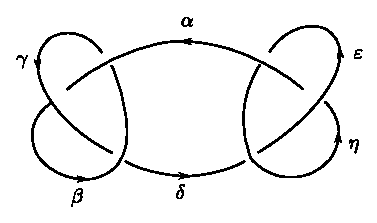
\includegraphics{vol44-fig/fig44-19.eps}
\end{figure}

For the definition of $\pi (T)$ and $\pi (\mathbb{R}^3 -
\overset{\circ}{T})$ let us choose a base point in $\mathbb{R}^2$ on the
boundary of $T$ in the portion above the arc $\alpha$. The method of
$\S 4$ gives the presentation of $\pi (\mathbb{R}^3 -
\overset{\circ}{T})$; 
$$
\pi (R^3 - \overset{\circ}{T}) = (\alpha, \beta, \gamma, \varepsilon, \eta 
; \beta \alpha = \alpha \gamma = \gamma \beta = \beta \delta, \eta\delta =
\varepsilon \eta = \alpha \varepsilon = \eta \alpha)  
$$

Setting $\beta \alpha = \sigma$ and $\eta \delta = \tau$ we get
\begin{gather*}
\beta = \sigma \alpha^{-1}, \gamma = \alpha^{-1} \sigma, \delta =
\alpha, \eta = \tau  \alpha^{-1}, \varepsilon = \alpha^{-1} \tau\\ 
\alpha^{-1} \sigma^2 \alpha^{-1} = \sigma, \alpha^{-1} \tau^2
\alpha^{-1} = \tau.  
\end{gather*}
Then one can take $\alpha$, $\sigma$, $\tau$ as generators and the
relations reduce to  
$$
\sigma^2 = \alpha \sigma \alpha, \tau^2 = \alpha \tau \alpha
$$
giving\pageoriginale 
$$
\pi (R^3 - \overset{\circ}{T}) = (\alpha, \sigma, \tau; \sigma^2 = \alpha
\sigma \alpha;  \tau^2 = \alpha \tau \alpha). 
$$
From these relations it follows that
\begin{gather*}
\sigma^3 \alpha = \alpha \sigma^3, \tau^3 \alpha = \alpha \tau^3 \\ 
\gamma \alpha \beta  = \alpha^{-1} \sigma \alpha\sigma \alpha^{-1} =
\alpha^{-2} \alpha \sigma \alpha  \sigma \alpha^{-1} = \alpha^{-2}
\sigma^3  \alpha^{-1} = \sigma^3 \alpha^{-3}\\ 
\varepsilon \alpha \beta = \alpha^{-1} \tau \alpha \tau \alpha^{-1} =
\alpha^{-2} \alpha \tau \alpha \tau \alpha^{-1} = \alpha^{-2} \tau^3
\alpha^{-1} = \tau^3 \alpha^{-3}	. 
\end{gather*}

The group $\pi (\partial T)$ is a free abelian group of two generators
for which we take the homotopy class of the meridian $m$ i.e. the
boundary of the disc bounding $T_+$ containing the base point and that
of $l$ the longitude formed by the fibre of $T$ passing through the base
point. The group $\pi (T)$ is infinite cyclic and in the homomorphism
$\pi (\partial T) \to \pi (T)$ induced by the inclusion $l$ goes to a
generator and $m$ goes to the identity element, the meridian of
$\partial T$ being homotopic to zero in $T$. On the other hand,
considering $\partial T$ as the boundary of $R^3 - \overset{\circ}{T}$,
the inclusion homomorphism $\pi (\partial T) \to \pi ( R^3 -
\overset{\circ}{T})$ takes $m$ onto $\alpha$ and $l$ onto the homotopy
class of a fibre of $\partial T$ which is  
$$
\chi = \gamma \alpha \beta \eta^{-1} \alpha^{-1} \varepsilon^{-1} =
\gamma \alpha \beta (\varepsilon \alpha \eta)^{-1} = \sigma^3
\tau^{-3} 
$$
as one deduces from Figure 2 and the above relations.

When the point $(e^{i \varphi}, s)$ describes a meridian of $T$,
$\varphi$ varying 0 to $2 \pi$ and $s$ remaining fixed in the
meridian $\psi = 0$ of $S^2$, $r_{k \varphi} (s)$ describes the great
circle of $S^2$ formed by the meridians $\psi = 0$ and $\psi = \pm
\pi$, which corresponds to a fibre\pageoriginale of $T$,
$k$-times. Consequently 
$g^k (e^{i \varphi}, s) = (e^{i \varphi}, r_{k \varphi} (s))$
describes a curve whose homotopy class is $ml^k$ and therefore the
homomorphism induced by $g^k$ takes $m$ onto $ml^k$ which in its turn
goes onto $\alpha \alpha^k = \alpha (\sigma^3 \tau^{-3} )^k$ by the
inclusion homomorphism.  

Then it results from (\ref{thm3.2}) that $G_k$ is obtained from $\pi (R^3 -
\overset{\circ}{T})$ by adding the relation 
$$
\alpha \chi^k = 1 
$$
and thus
$$
G_k = \pi (M_k) = (\alpha, \sigma, \tau; \sigma^2 = \alpha \sigma
\alpha, \tau^2 = \alpha \tau \alpha, \alpha = (\tau^3
\sigma^{-3})^k). 
$$

For $k = 0$ we have $\alpha = 1$ and consequently $\sigma = \tau =1$
and $G_o$ reduces to the unit element agreeing with the fact that $M_0
= \mathbb{R}^3$. Also let us remark that $G_k$ and $G_{-k}$ are
isomorphic: since $(\sigma^3 \tau^{-3} )^{-k} = (\tau^3 \sigma^{-3})^k$
the permutation of $\sigma$ and $\tau$ realises the isomorphism. 

Now it remains to prove that for $k = 0, 1, 2,\ldots$ the groups
$G_k$ are mutually non- isomorphic. This is an immediate consequence of
the following proposition which we are going to prove. 

\begin{prop*}
There are exactly two minimal invariant subgroups $N$ and $N'$ of
  $G_k$ such that $G_k / N$ and $G_k / N'$ admit faithful
  representations into the group $G$ of non-euclidean motions or (in
  the exceptional case $k = 1$) into $S0 (3)$. The maximum of the
  orders of elements of finite order in $G_k / N$ and $G_k / N'$ is
  $6k -1$ for one and $6k +1$ for the other. 
\end{prop*}

\begin{proof}
Let\pageoriginale $\alpha \to A$, $\sigma \to S$, $\tau \to T$ be a
non-trivial representation of $G_k$ into $G$ or into $S0(3)$. We have
three relations   
$$
S^2 = ASA, T^2 = ATA, A = (S^3 T^{-3})^k
$$
and 
$$
S^3 A = AS^3, T^3 A = AT^3
$$
\end{proof}

Under these circumstances one cannot have $A = 1$ for then the
representations would be trivial. In virtue of the properties of $G$
and of $S0(3)$, if $S^3 \neq 1$ the relation $S^3 A = AS^3$ gives $AS
= SA$ which in view of the relation $S^2 = ASA$ gives $S =
A^2$. Likewise if $T^3 \neq 1$ we have $T = A^2$. One can have neither
$S^3 \neq 1$ and $T^3 \neq 1$ nor $S^3 = T^3 =1$ since in these cases
$S^3 = T^3$ and then $A=1$ and the representation would be trivial. 

If $S^3 = 1$ and $T^3 \neq 1$ one has $T = A^2$ and one is reduced to
the representation of the quotient of $G_k$ by the relation $\sigma^3
=1$ and $\tau = \alpha^2$, i.e. $N$ being the corresponding invariant
subgroup, to the representation of  
$$
G_k / N = (\alpha, \sigma; \sigma^3 = (\alpha \tau)^2 = \alpha^{6k-1} =1)
$$
If $S^3 \neq 1$ and $T^3 = 1$ one is reduced to the representation of
$G_k /N' = (\alpha, \tau ; \tau^3 = (\alpha \tau)^2 = \alpha ^{6k +1}
=1)$. 

These are the groups $(2,3,6k -1)$ and $(2,3,6k+1)$ which, as we have
already seen, admit a faithful representation into $G$ with the
exception of (2, 3, 5) which is the alternating group of 5 letters
and which admits a faithful representation onto the icosahedral group
in $SO(3)$. 

Thus\pageoriginale $6k +1$ is the maximum of orders of elements of
finite order for homomorphic images of $G_k$ in $G$. This is
sufficient to ensure that the groups $G_k (k \geq 0)$ are all
distinct.  

\medskip
\noindent
\textbf{References.} Other constructions of contractible manifolds
analogous to the $V_{2k}$ have been Mazur and Po\'enaru. 

\begin{thebibliography}{99}
\bibitem{key1} B. Mazur. A note on some contractible 4-manifolds. Annals of
Math. 73(1961) pp 221-228.  

\bibitem{key2} V. Po\'enaru. Les decompositions de l'hypercuble en product
topologique. Bull. Sco. Math. France 88, 1960, pp 113-129. 

\bibitem{key3} G. de Rham. Factorisations topologiques du disque \'a cinq
dimensions. Seminarie de topologic et geom\'etric diff\'erentielle derige
par Ch. Ehresmann Vol, III (1960 - 1961- 1962), Institut Henri
Poincar\'e, Paris. 

\bibitem{key4} G. de Rham. Involutions topologiques de $S^4$ Seminere dell' Instituto
Nazionale di alta Mathematica 1962-63, pp 725-736. 
\end{thebibliography}

\newpage

\begin{center}
\textbf{\Large{Addendum}}
\end{center}

As\pageoriginale Mr. G.A. Swarup has kindly pointed out to me (letter
March 1968) is follows from the work of H. Gluck ``The embedding of
two-spheres in the four sphere'' (Trans. of the
Am. Math. Soc. Vol. 104, 1962, pp 308 - 333) that $V_1$ and
consequently $V_{2k + 1}$ is also homeomorphic to $\mathbb{R}^4$. The
proof is sketched here.  

Given a continuous map $\gamma : S^1_0 \to  SO (3)$ let us say that
\textit{the homeomorphism} $h: \partial A \to \partial A = \partial
B$ defined by $h(e^{i \varphi}, s) = (e^{i \varphi}, r (s))$ where $r =
\gamma (e^{i \varphi}) \in SO (3)$ is the rotation of $S^2$, the image
of $e^{i \varphi} \in S^1_0$ by $\gamma$ \textit{is associated to
  $\gamma$}. Then one can state the following generalisation of the
proposition \ref{prop1}. 

\textit{If $h_1, h_2 : \partial A \to \partial B$ are homeomorphisms
  associated to two homotopic maps $\gamma_1, \gamma_2: S^1_O \to
  SO (3)$ then $V(h_1)$ and $V(h_2)$ are homeomorphic.}  

If fact, let $r_1 = \gamma_1 (e^{i \varphi})$, $r_2 = \gamma_2 (e^{i
  \varphi})$; it results from the hypothesis that the map $\gamma$
given by $r^{-1}_1 \circ r_2$ is homotopic to zero. The homeomorphism
associated to $\gamma$ is $f = h^{-1}_1 \circ h_2$  so that $h_2 = h_1
\circ f$ and the rest of the proof is as in proposition \ref{prop1}, the role of
$g^2$ being played here by $f$. 

Now let us denote by $\rho_{\alpha}$ the rotation of $S^2$ through an angle 
$\alpha$ around the axis of the poles which changes $S(\theta, \psi)$ into
$S(\theta, \gamma + \alpha)$. The two maps $\gamma_1$ and $\gamma_2$
defined by $\gamma_1 (e^{i \varphi}) = r_\varphi$ and\pageoriginale
$\gamma_2 (e^{i \varphi})=\rho_\varphi$ are 
homotopic. Let $\alpha = \alpha (\varphi)$ be a continuous function
monotonically increasing from 0 to $2 \pi$ in the interval $- \in
\leq \varphi \leq \in$, $\in$ being a positive number less than
$\pi$. The map $\gamma: S^1_o \to SO (3)$ defined by setting $\gamma
(e^{i \varphi} ) = \rho_\alpha$ if $|\varphi| \leq \varepsilon$ and
$\gamma (e^{i \psi})=$ identity if $\in \leq | \varphi | \leq \pi$ is
homotopic to 
$\gamma_2$ and hence to $\gamma_1$. If $h$ is the homeomorphism
associated to $\gamma$, as $g$ is associated to $\gamma_1$, it follows
from the above proposition that $V_1 = V(g)$ is homeomorphic to
$V(h)$. Thus one is reduced to prove that $V(h)$ is homeomorphic to
$\mathbb{R}^4$. For this \textit{it is enough to prove that $h:
\theta B \to \partial B$ can be extended into a homeomorphism}
$\tilde{h}: B \to B$ since one will then obtain a homeomorphism of
$\mathbb{R}^4$ onto $V(h)$ by taking identity in $A$ and $\tilde{h}$
in $B$. 

To make this extension let us remark, to start with, that the point
$h(e^{i \varphi}, s)$ is obtained from the point $(e^{i \varphi}, s)$ by
a rotation through an angle $\alpha = \alpha (\varphi)$ around
$\mathbb{R}^2$. In fact, if $s = s (\theta, \varphi)$, then $h(e^{i
  \varphi}, s) = (e^{i \varphi}, s^1)$ with $s' = \rho_\alpha (s) =
s(\theta, \psi + \alpha)$. Now let us consider the knot formed in
$\mathbb{R}^3$ by a fibre $e^{i \varphi } \alpha S^1$ of $\delta
T$. By the method of  Seifert (Uber des geschlecht von knoten,
Math. arn. vol. 10, pp 571-592) one can construct a surface
$F_{\varphi}$ which is compact, orientable, differentiable and
contained in $R^3 - \overset{\circ}{T}$ and is bounded by this fibre $e^{i
  \varphi} \times S^1$. One can construct it in such a way that it is 
symmetric relative to $\mathbb{R}^2$. Moreover, for sufficintly small
$\varepsilon > 0$, one can make this construction for every $\varphi$ with
$|\varphi| \leq \varepsilon$ in such a way that the set of
surfaces\pageoriginale $F_{\varphi}$ from a fibration of a three
dimensional manifold which 
is contained in $R^3 - \overset{\circ}{T}$ and is bounded by
$F_{\varepsilon}$, $F_{- \varepsilon}$ and the portion of $\partial T =
S_\circ^1 \times S^1$ corresponding to the arcs $|\varphi| \leq \varepsilon$
of $S^1_\circ$. By rotation around $\mathbb{R}^2$, $F_{\varphi}$ generates a
three dimensional manifold $W_{\varphi} \subset B$. Let $B'$ be the
union of $W_{\varphi}, |\varphi| \leq \varepsilon$. This is a
manifold fibred by $W_{\varphi}$. The homeomorphism $\tilde{h} : B \to
B$ which reduces to the identity outside $B'$ and coincides on
$W_{\varphi} \subset B'$ with the rotation through the angle $\alpha =
\alpha (\varphi)$ around $\mathbb{R}^2$ gives a desired extension of
$h$ to $B$. 
